\documentclass[11pt,a4paper]{article}

% ── Packages ──────────────────────────────────────────────────────────
\usepackage[utf8]{inputenc}
\usepackage[T1]{fontenc}
\usepackage{amsmath,amssymb,amsfonts}
\usepackage{booktabs}
\usepackage{graphicx}
\usepackage[colorlinks=true,linkcolor=blue!60!black,citecolor=blue!60!black,urlcolor=blue!60!black]{hyperref}
\usepackage{cleveref}
\usepackage{algorithm}
\usepackage{algpseudocode}
\usepackage{tikz}
\usepackage{pgfplots}
\pgfplotsset{compat=1.18}
\usepackage[margin=1in]{geometry}
\usepackage{microtype}
\emergencystretch=3em
\hbadness=5000
\vbadness=5000
\usepackage{natbib}
\bibliographystyle{plainnat}
\usepackage{xcolor}
\usepackage{subcaption}
\usepackage{multirow}

\definecolor{condA}{HTML}{4C72B0}
\definecolor{condB}{HTML}{DD8452}
\definecolor{condC}{HTML}{55A868}
\definecolor{ablOracle}{HTML}{C44E52}
\definecolor{ablRandom}{HTML}{8172B3}
\definecolor{ablUniform}{HTML}{937860}

% ── Title ─────────────────────────────────────────────────────────────
\title{%
  Computed Targets and the Middleman Protocol:\\
  Mathematical Guardrails and Channel Removal\\
  for LLM Negotiators in Multi-Issue Bargaining%
}

\author{%
  Thor Matthiasson\\
  Independent Researcher\\
  New Haven, Connecticut, USA\\
  \texttt{thor@aiwiththor.com}
}

\date{May 2026}

% ══════════════════════════════════════════════════════════════════════
\begin{document}
\maketitle

% ── Abstract ──────────────────────────────────────────────────────────
\begin{abstract}
Aligned LLMs negotiate cooperatively by default. We test whether providing them with explicit opponent-preference information improves their bargaining outcomes, and find the opposite: text-based strategic advice consistently \emph{reduces} buyer surplus, an effect we read as alignment-induced cooperation bias though we do not establish it causally. Replacing the advice with a numeric target proposal computed by a small external module (an 11K-parameter NegotiationGRU) recovers and exceeds the unassisted baseline.

Scaled experiments ($N\!=\!200$, randomized opener, Claude 3.5 Haiku) decompose the effect into anchoring defense ($+7.1$pp, opener-dependent), a residual GRU-conditioned share edge ($+3.0$pp, opener-independent), and variance collapse ($2.3$--$9.9\times$, format-driven); eight of ten pairwise Holm--Bonferroni-corrected comparisons reach $p\!=\!0.001$. An Oracle ablation shows the cooperative-blend formula mechanically converges to Nash bargaining under accurate weights, yielding the highest Pareto efficiency ($79\%$) but the lowest buyer share ($49.5\%$)---a property of the chosen blend, not a fundamental law. Replication across eight models from five labs (Haiku, Opus 4.6, GPT-5, Gemini 3 Pro/Flash, Grok 3/Mini, DeepSeek R1) yields a three-tier taxonomy---\emph{scaffold-responsive} ($+3$--$7$pp, $2$--$3\times$ collapse), \emph{collapse-only} (variance reduction without surplus shift), and \emph{no detectable effect at $N\!=\!50$} for Opus 4.6 and Gemini Pro (power-limited)---with the consistency gap predicted by baseline negotiation stochasticity, not model size. Cross-model: a cheap Haiku-with-scaffold buyer keeps a $5.2$pp edge against Grok 3 but loses $0.9$--$2.1$pp to frontier sellers, and the variance-collapse property disappears ($\pm 11.3$--$20.3\%$).

\textbf{We then show that the 11{,}078-parameter GRU reduces, behaviorally, to a $15$-line analytical estimator with one tunable scalar (\Cref{sec:bias_scalar})}: its weight predictions on LLM trajectories are at chance, variance collapse derives entirely from the directive format, and the residual share gain reduces to a single bias parameter. The architecture is best read as a structured numeric sub-agent with a tunable aggression knob, not a learned opponent model in the Theory-of-Mind sense. A stronger architectural intervention removes the language channel entirely: each side submits structured numeric inputs to a neutral middleman protocol. In offline replay, the $N\!=\!200$ weight pairs routed through Nash bargaining and the cooperative-blend formula reach $96\%$ and $91\%$ Pareto efficiency respectively, breaking the $79\%$ language-channel ceiling of the Oracle condition, and replaying the four cross-model match-ups collapses the $7.3$pp buyer-share spread to $\le\!0.001$pp; a live $N\!=\!50$ Haiku-vs-Haiku LLMIO test confirms the cooperative-blend $50/50$ split is structural and robust to translation noise (per-game drift $0.001$ vs.\ Nash's $0.181$), with cross-model LLMIO as future work. Appendix~A reports a 6.5K-parameter neural policy that reaches $100\%$ deal rate at the lowest variance observed; because it rests on a single RWR temperature and lacks the GRU-mask control, we treat it as hypothesis-generating rather than load-bearing.
\end{abstract}

% ── 1  Introduction ───────────────────────────────────────────────────
\section{Introduction}
\label{sec:intro}

Large language models are increasingly deployed as autonomous negotiation agents~\citep{fu2023improving,abdelnabi2024cooperation}, and recent at-scale deployments are starting to surface the practical consequences. Anthropic's \emph{Project Deal}~\citep{anthropic2026projectdeal}---a real-money agent-to-agent marketplace with 69 participants and 186 deals---reports two findings that closely parallel ours: (i) instructing agents ``to negotiate aggressively had negligible statistically significant effects,'' echoing our finding that text-based strategic advice backfires, and (ii) users represented by stronger models (Opus) systematically extract more surplus than users with weaker models (Haiku), without the disadvantaged users perceiving the gap (fairness ratings 4.05 vs.\ 4.06). Their work demonstrates the problem at deployment scale; we contribute the mechanistic decomposition and an architectural remedy.

Their natural-language fluency makes LLMs compelling candidates for multi-issue bargaining, where integrative potential depends on identifying and exploiting asymmetric preferences. Yet language fluency alone does not confer strategic competence. An agent must infer what the opponent values, decide where to concede and where to hold firm, and communicate offers that advance its position---three capabilities with fundamentally different computational requirements.

Prior work on LLM negotiation typically conflates these roles: the same model that generates natural language also performs belief inference and strategic planning. We argue this conflation is a design error when the LLM is RLHF-aligned. Alignment training biases the model toward cooperative, other-regarding behavior~\citep{perez2022discovering}, which is adaptive in conversational assistance but maladaptive in competitive bargaining.

Our contributions are:

\begin{enumerate}
\item We demonstrate that \textbf{text-based strategic advice backfires}: providing an aligned LLM with opponent preference information consistently reduces its negotiation surplus. We treat the alignment-as-cause story as observational rather than causally established (\Cref{sec:limitations}).
\item We introduce a \textbf{Computed-Target Architecture} that decouples strategy from communication: a small GRU-based strategic module computes a numeric target proposal, and the LLM executes it in natural language.
\item Through scaled experiments ($N = 200$, randomized opener), we decompose the computed-target effect into anchoring defense ($+7.1$pp) and a residual GRU-conditioned share edge ($+3.0$pp) that persists when the anchoring confound is removed. Pairwise permutation tests (10K resamples, two-sided) with Holm--Bonferroni correction across the pre-specified family of $\binom{5}{2}\!=\!10$ ablation comparisons (\Cref{tab:holm}) give $p_{\text{Holm}} = 0.001$ for eight of ten pairs, including GRU vs.\ Random ($+2.8$pp), GRU vs.\ Uniform ($+5.8$pp), GRU vs.\ A ($+3.0$pp), and Oracle vs.\ GRU ($-5.7$pp), so the residual edge survives multiple-comparisons correction.
\item Full ablations ($N = 200$) document an \textbf{Oracle ablation}: with accurate opponent weights the cooperative blend formula (\Cref{eq:blend}) mechanically converges toward Nash bargaining, yielding $9.9\times$ variance collapse, $79\%$ Pareto efficiency, and the lowest buyer share ($49.5\%$). We frame this as a property of the chosen blend, not a fundamental law.
\item We identify \textbf{variance collapse} ($1.1$--$2.8\times$ across the eight-model panel; $2.3$--$9.9\times$ for the Haiku ablation gradient at $N\!=\!200$, reaching $9.9\times$ at the Oracle weight source) as the architecture's most practically significant property, driven by the directive \emph{format} rather than prediction accuracy.
\item Multi-model replication (\Cref{sec:multimodel}) suggests a three-tier taxonomy: \emph{scaffold-responsive} (stochastic models, $+3$--$7$pp), \emph{collapse-only} ($1.4$--$1.6\times$ variance reduction), and \emph{no detectable effect at $N\!=\!50$} (Opus 4.6, Gemini Pro). The strongest predictor of computed-target effectiveness is baseline negotiation stochasticity, not model capability.
\item \textbf{Cross-model experiments} show a cheap Haiku buyer with opponent model captures $55\%$ surplus against Grok~3 but cannot overcome the capability gap against Opus~4.6, GPT-5, or Gemini~Pro.
\item We introduce a \textbf{Middleman Protocol} architecture in which the LLM-to-LLM language channel is replaced by a structured numeric protocol; LLMs act as I/O layers that translate user intent in and explain outcomes out, but never converse. Offline replay of the $N\!=\!200$ randomized-opener weight pairs through Nash bargaining and the paper's cooperative-blend formula captures $96\%$ and $91\%$ of joint surplus respectively, breaking the $79\%$ Pareto ceiling of the Oracle condition. Replay of the four cross-model match-ups collapses the $7.3$pp surplus spread to $\le 0.001$pp (\Cref{sec:middleman}), and the live $N\!=\!50$ LLMIO test confirms that the cooperative-blend protocol's $50/50$ split is structural and robust to translation noise. We interpret these results as evidence consistent with a channel-mediated account of the cross-model gap.
\item Appendix~A reports a \textbf{follow-on neural distillation study}: a 6.5K-parameter policy trained via behavioral cloning and reward-weighted regression on 660 live LLM games reaches 100\% deal rate and reproduces the architecture's low-variance regime. We treat the RWR $\tau=0.2$ result as hypothesis-generating rather than established, because it rests on a single temperature setting and lacks the GRU-mask control (\Cref{sec:limitations}).
\item In a diagnostic re-analysis we show that the trained NegotiationGRU's weight predictions on LLM trajectories are at chance and its $11{,}078$ parameters can be replaced by a $15$-line analytical estimator with one tunable scalar; variance collapse derives entirely from the directive format and the residual share gain reduces to a bias parameter (\Cref{sec:bias_scalar}). We recommend reading the architecture as a structured numeric sub-agent.
\end{enumerate}

% ── 2  Related Work ───────────────────────────────────────────────────
\section{Related Work}
\label{sec:related}

\paragraph{Multi-issue negotiation.}
The multi-issue framework dates to \citet{raiffa1982art}. Automated negotiation agents in the ANAC competition~\citep{baarslag2015anac} typically use opponent modeling via frequency analysis or Bayesian estimation~\citep{baarslag2013acceptance}. Our NegotiationGRU serves a similar role but operates on raw behavioral features.

\paragraph{LLM negotiation agents.}
End-to-end neural negotiation dialogue was pioneered by \citet{lewis2017deal} on a multi-issue allocation game; \citet{he2018decoupling} subsequently showed that \emph{decoupling} strategic dialogue acts from natural-language generation outperforms end-to-end models, an architectural pattern our Computed-Target and Middleman designs extend to RLHF-aligned LLMs in continuous-issue bargaining. \citet{fu2023improving} use GPT-4 for price negotiation with chain-of-thought reasoning. \citet{abdelnabi2024cooperation} study multi-agent LLM bargaining and find cooperation biases similar to those we document. \citet{gandhi2023strategic} find that LLMs struggle with strategic reasoning in game-theoretic settings. \citet{bianchi2024llm} benchmark LLM negotiators across multiple games and find systematic underperformance vs.\ human or rule-based opponents; \citet{davidson2024evaluating} evaluate language model agency through structured negotiations and document capability-driven asymmetries that closely parallel our cross-model findings (\Cref{sec:crossmodel_asym}). \citet{bakhtin2022human} (Cicero) extends the decoupling pattern to human-level Diplomacy by pairing language models with an explicit strategic planning module. Our work goes further by documenting that, even with accurate external intelligence supplied as text, surplus drops below the unassisted baseline---a pattern we read as evidence of the cooperation prior identified by \citet{perez2022discovering,sharma2023sycophancy} though we treat the alignment-as-cause story as observational rather than causally established (\Cref{sec:limitations})---and quantifies the contribution of numeric directive format vs.\ opponent-model accuracy via ablation.

\paragraph{Theory of Mind in AI agents.}
Machine Theory of Mind~\citep{rabinowitz2018machine} trains neural networks to predict agent behavior. \citet{wang2022tom2c} extend ToM to multi-agent communication and cooperation settings. Our NegotiationGRU is a specialized ToM model, but our ablation results show that the ToM component is less important than the structured directive format.

\paragraph{Alignment-induced cooperation and sycophancy.}
RLHF and constitutional training reliably produce LLMs biased toward cooperative, agreeable, and other-regarding behavior~\citep{perez2022discovering}. \citet{sharma2023sycophancy} document a robust sycophancy phenomenon---LLMs adapt their stated positions toward perceived user expectations even when this contradicts evidence. \citet{park2024ai} survey deception capabilities and find that frontier LLMs already engage in strategic misrepresentation in adversarial games. We read our text-advice failure (\Cref{sec:text_fail}) as a competitive-bargaining instance of the same prior: the model interprets opponent-preference information as social context for accommodation rather than tactical input for exploitation. We treat this reading as observational rather than causally established (\Cref{sec:limitations}).

\paragraph{Centaur / neuro-symbolic systems.}
The term ``Centaur'' originates in chess~\citep{kasparov2017deep}. More broadly, neuro-symbolic integration~\citep{garcez2023neurosymbolic} and tool-augmented LLMs~\citep{schick2023toolformer} pair neural language models with structured external modules. Our architecture follows this pattern but our ablation results complicate the narrative: the ``engine's'' predictions contribute less than the directive format itself.

% ── 3  Methods ────────────────────────────────────────────────────────
\section{Methods}
\label{sec:methods}

\subsection{Negotiation Environment}
\label{sec:env}

Two agents (buyer and seller) negotiate a B2B SaaS contract over five continuous variables $v_i \in [0.05, 0.95]$:

\begin{center}
\begin{tabular}{llcc}
\toprule
Variable & & Buyer prefers & Seller prefers \\
\midrule
Price & $v_1$ & Low & High \\
Contract length & $v_2$ & Long & Short \\
Payment terms & $v_3$ & Slow & Fast \\
SLA tier & $v_4$ & High & Low \\
Data rights & $v_5$ & Client & Vendor \\
\bottomrule
\end{tabular}
\end{center}

Each agent has hidden utility weights $\mathbf{w} \in \Delta^4$ sampled from $\text{Dirichlet}(\alpha)$, $\alpha = 1.0$. Utility is:
\begin{equation}
U(\mathbf{v}, \mathbf{w}, \text{role}) = \sum_{i=1}^{5} w_i \cdot \tilde{v}_i, \qquad \tilde{v}_i = \begin{cases} v_i & \text{if direction}_i = +1 \\ 1 - v_i & \text{if direction}_i = -1 \end{cases}
\label{eq:utility}
\end{equation}
Agents alternate proposals for up to $R_{\max} = 8$ rounds. No deal yields $U = 0$ for both. Initial experiments use seller-first opening; all scaled experiments ($N = 200$) and multi-model replication use randomized opener to control for anchoring (see \Cref{sec:opener}).

\subsection{NegotiationGRU}
\label{sec:gru}

The NegotiationGRU predicts an opponent's utility weights $\hat{\mathbf{w}}_{\text{opp}}$ from an observation sequence $\mathbf{x}_{1:T}$, where each $\mathbf{x}_t \in \mathbb{R}^{11}$:

\paragraph{Feature vector (11D).}
\begin{itemize}
\item \textbf{Dims 0--4:} Per-variable cumulative concession from the opponent's opening proposal.
\item \textbf{Dim 5:} Proposal centroid (mean of the 5D proposal).
\item \textbf{Dim 6:} Round fraction $t / R_{\max}$.
\item \textbf{Dim 7:} Utility delta between opponent's last two proposals.
\item \textbf{Dim 8:} Concession magnitude ($\ell_2$ norm of proposal delta).
\item \textbf{Dim 9:} Variable spread (std of cumulative concessions).
\item \textbf{Dim 10:} Max concession channel ($\arg\max$ of cumulative concession / 4).
\end{itemize}

\paragraph{Architecture (11,078 params).}
Encoder Linear($11\!\to\!64$)$\to$LayerNorm$\to$GELU$\to$Linear($64\!\to\!32$); GRU($32\!\to\!32$); dual heads: weight head Linear($32\!\to\!32$)$\to$Linear($32\!\to\!5$) with softmax, threshold head Linear($32\!\to\!16$)$\to$Linear($16\!\to\!1$) with sigmoid. Read-out at time-step $\lfloor 3T/4 \rfloor$. Parameter breakdown: encoder $2{,}976$ + GRU $6{,}336$ + weight head $1{,}221$ + threshold head $545$ $=$ $11{,}078$.

\paragraph{Training.}
20{,}000 \textsc{HeuristicNegotiator}-vs-\textsc{HeuristicNegotiator} matches, $\text{Dirichlet}(0.7)$ weights, noise $\sigma = 0.01$. The \textsc{HeuristicNegotiator} is a hand-coded baseline that on each round (i) computes its current target $v_i$ from its own weights via the same blend in \Cref{eq:blend} with a calibrated aggression schedule, (ii) concedes toward its opponent's last offer at a per-variable rate $(1 - w_i)^2 \cdot r_\text{base}$ (low-weight variables move faster), and (iii) accepts when the offered utility exceeds a deadline-decaying threshold; full implementation in \texttt{heuristic\_om.py} of the data packet. \textbf{On heuristic test data:} cosine similarity 0.988, top-1 accuracy $89.8\%$, MAE $0.034$.

\paragraph{Reading order.} We present the architecture as designed and trained. \Cref{sec:bias_scalar} returns to ask which components are actually load-bearing on LLM trajectories and shows that the 11K-parameter NegotiationGRU is functionally a $15$-line analytical estimator with one tunable scalar. The GRU's accuracy numbers above describe its behavior on the heuristic distribution it was trained on; whether this generalizes to LLM behavior is a question we test, not assume.

\subsection{Computed-Target Architecture}
\label{sec:computed}

Given the agent's own weights $\mathbf{w}_{\text{me}}$ and \emph{some} opponent weight estimate $\hat{\mathbf{w}}_{\text{opp}}$ (from GRU, oracle, random, or uniform---see \Cref{sec:ablation}), we compute:

\begin{equation}
\text{target}_i = \beta_i \cdot \text{ideal}_i^{\text{me}} + (1 - \beta_i) \cdot \text{ideal}_i^{\text{opp}}
\label{eq:target}
\end{equation}

where $\text{ideal}_i^{\text{me}}, \text{ideal}_i^{\text{opp}} \in \{0.10, 0.90\}$ are the extreme-preference endpoints and:

\begin{equation}
\beta_i = \frac{w_{\text{me},i}}{w_{\text{me},i} + \hat{w}_{\text{opp},i} + \epsilon} \cdot a + (1 - a) \cdot 0.5, \qquad a = \max(0.55,\; 0.80 - 0.30 \cdot t/R_{\max})
\label{eq:blend}
\end{equation}

The aggression parameter $a$ decays from 0.80 toward 0.55 as the deadline approaches. The computed target is injected into the LLM's system prompt as a concrete directive with expected utility and acceptance guidance.

Note that even with $\hat{\mathbf{w}}_{\text{opp}} = [0.2, 0.2, 0.2, 0.2, 0.2]$ (uniform, zero information), the formula still produces a differentiated target because it uses the agent's \emph{own} known weights $\mathbf{w}_{\text{me}}$ to determine where to push harder.

\subsection{LLM Agent Design}
\label{sec:llm}

Each LLM agent receives a system prompt with its role, its own utility weights, preference directions, and (in OM conditions) the computed-target directive. Agents produce structured JSON: \texttt{internal\_monologue}, \texttt{message}, \texttt{formal\_proposal} (5D), and \texttt{action} (offer/accept). All models are accessed via OpenRouter. Primary experiments use Claude 3.5 Haiku; multi-model replication (\Cref{sec:multimodel}) spans eight models from five labs.

Two mechanisms ensure deal closure: deadline pressure warnings in rounds 6--8, and a hard accept override in the final round if utility $> 0.15$.

\subsection{Experimental Conditions}
\label{sec:conditions}

\begin{table}[h]
\centering
\caption{Experimental conditions.}
\label{tab:conditions}
\begin{tabular}{clccl}
\toprule
Cond. & Name & Buyer OM & Seller OM & Tests \\
\midrule
A & Baseline & \texttimes & \texttimes & Unassisted LLM negotiation \\
B & Unilateral & \checkmark & \texttimes & One-sided computed target \\
C & Bilateral & \checkmark & \checkmark & Both sides use computed targets \\
\bottomrule
\end{tabular}
\end{table}

\subsection{Ablation Conditions}
\label{sec:ablation}

To disentangle the effect of the \emph{numeric directive format} from the \emph{accuracy of opponent modeling}, we run Condition~B with four different opponent-weight sources in the computed-target formula:

\begin{table}[h]
\centering
\caption{Ablation conditions for the opponent weight source in Condition~B ($N = 50$ each, same seed).}
\label{tab:ablation_design}
\begin{tabular}{lll}
\toprule
Source & $\hat{\mathbf{w}}_{\text{opp}}$ & Tests \\
\midrule
\textbf{GRU} & NegotiationGRU prediction & Full system (default) \\
\textbf{Oracle} & True opponent weights & Upper bound on ToM \\
\textbf{Random} & $\text{Dirichlet}(1.0)$ draw & Noise control \\
\textbf{Uniform} & $[0.2, 0.2, 0.2, 0.2, 0.2]$ & Zero-information (self-knowledge only) \\
\bottomrule
\end{tabular}
\end{table}

% ── 4  Results ────────────────────────────────────────────────────────
\section{Results}
\label{sec:results}

\subsection{Motivation: The Failure of Text-Based Advice}
\label{sec:pivot}

Before presenting our main results, we document the failure of the naive approach---providing strategic intelligence as natural-language advice---which motivates the computed-target architecture.

\paragraph{Text-based advice backfires.}
\label{sec:text_fail}
Our initial design generated text briefings from GRU predictions. Across three framing variants, the OM-equipped buyer consistently performed \emph{worse} than the unassisted baseline:

\begin{table}[h]
\centering
\caption{Buyer surplus share under text-based advice in the earlier pilot setup that motivated the main experiments. All variants fall \emph{below} the unassisted baseline; the $42.4\%$ baseline here is a within-table reference and should not be compared directly to the later standardized $N\!=\!50$ seller-first panel in \Cref{tab:results}.}
\label{tab:text_fail}
\begin{tabular}{lc}
\toprule
Text-advice variant & B buyer share \\
\midrule
Directional (``hold firm / concede'') & 38.6\% \\
Strong directional (``push HIGHER / LOWER'') & 33.7\% \\
Exploitation framing (``FREE GIVEAWAY / REFUSE'') & 40.7\% \\
\midrule
\emph{Unassisted baseline (A)} & \emph{42.4\%} \\
\bottomrule
\end{tabular}
\end{table}

\paragraph{The Negotiator's Dilemma.}
\label{sec:dilemma}
The failure pattern is consistent with an alignment-induced cooperation trigger (an interpretation we treat as observational rather than causally established; see \Cref{sec:limitations}). Internal monologue analysis suggests LLMs interpret opponent preference information as an invitation to accommodate. We illustrate with one representative excerpt; we have not coded transcripts at scale, so this is qualitative motivation rather than systematic evidence:

\begin{quote}
\small
\emph{``The model indicates the opponent values price highly. I should be understanding of their position on price and focus on finding mutually beneficial trade-offs...''}
\end{quote}

This resembles the Negotiator's Dilemma~\citep{lax1986manager}---the tension between creating and claiming value---reproduced autonomously. A preliminary test with Llama~3.3 70B (less aggressively aligned) showed qualitatively similar cooperation patterns, though baseline aggressiveness varied; we do not include these results as they were not run at sufficient scale. We propose, but do not causally establish, that alignment training functions here as a \emph{strategic constraint}: it biases the model toward cooperative, other-regarding behavior regardless of the information it receives. An alternative reading is that numeric directives are simply less ambiguous than text, and the observed effect reflects instruction clarity rather than alignment bypass; we discuss this in \Cref{sec:limitations}. Either way, an architectural fix---bypass the language channel with numeric directives---is empirically motivated.

\paragraph{The sim-to-real gap.}
Fine-tuning the GRU on LLM game telemetry (50 matches, $\text{lr} = 10^{-4}$, gradient clipping) produced 15\% top-1 accuracy---\emph{below} the 20\% random baseline. LLM concession patterns carry no weight-proportional signal in the per-variable features. This motivated the move to computed targets, and the GRU accuracy results in \Cref{tab:gru_accuracy} confirm the distributional mismatch persists even without fine-tuning.

\subsection{\texorpdfstring{Primary Results ($N = 50$)}{Primary Results (N = 50)}}

\begin{table}[t]
\centering
\caption{Negotiation outcomes by condition ($N = 50$ per condition, seller-first opening). Values are means $\pm$ sample standard deviations. Bold indicates best value per metric. All conditions achieved 100\% deal rate.}
\label{tab:results}
\begin{tabular}{lccc}
\toprule
Metric & A (No OM) & B (Buyer OM) & C (Both OM) \\
\midrule
Buyer utility       & 0.477 $\pm$ 0.087 & \textbf{0.599 $\pm$ 0.042} & 0.490 $\pm$ 0.042 \\
Seller utility      & 0.570 $\pm$ 0.089 & 0.477 $\pm$ 0.051 & \textbf{0.575 $\pm$ 0.033} \\
Joint surplus       & 1.047 & \textbf{1.076} & 1.065 \\
Pareto efficiency   & 75\% $\pm$ 6\% & \textbf{77\% $\pm$ 6\%} & 76\% $\pm$ 5\% \\
Buyer surplus share & 45.6\% $\pm$ 7.9\% & \textbf{55.7\% $\pm$ 3.0\%} & 46.0\% $\pm$ 2.6\% \\
Avg rounds          & 6.6 & 6.9 & 7.0 \\
\bottomrule
\end{tabular}
\end{table}

\Cref{tab:results} presents the full $N = 50$ results with seller-first opening. The computed-target GRU produces a \textbf{$+10.1$ percentage-point shift in buyer surplus share} (A: $45.6\%$ $\to$ B: $55.7\%$), corresponding to a $+25.6\%$ increase in absolute buyer utility ($0.477 \to 0.599$).

Joint surplus increases from $1.047$ (A) to $1.076$ (B), a $+2.8\%$ gain, and Pareto efficiency rises from $75\%$ to $77\%$. In Condition~C (bilateral), buyer share returns to $46.0\% \pm 2.6\%$ while joint surplus ($1.065$) and Pareto efficiency ($76\%$) remain elevated, consistent with the cooperative game theory prediction that mutual rationality expands the feasible set~\citep{nash1950bargaining}.

Note the dramatically lower variance in Conditions B ($\pm 3.0\%$) and C ($\pm 2.6\%$) compared to A ($\pm 7.9\%$): the computed-target directive regularizes LLM behavior. However, the seller-first opening creates an anchoring confound that inflates the apparent A$\to$B effect; we address this in \Cref{sec:opener}.

\subsection{GRU Accuracy on LLM Trajectories}
\label{sec:gru_accuracy}

A critical question: does the GRU actually predict opponent weights accurately when observing LLM (rather than heuristic) behavior?

\begin{table}[h]
\centering
\caption{NegotiationGRU prediction accuracy on heuristic vs.\ LLM behavioral data. The pretrained GRU is evaluated without fine-tuning on LLM trajectories.}
\label{tab:gru_accuracy}
\begin{tabular}{lcc}
\toprule
Metric & Heuristic data & LLM trajectories ($N = 300$) \\
\midrule
Cosine similarity & \textbf{0.988} & 0.638 \\
Top-1 accuracy & \textbf{89.8\%} & 24.3\% \\
Top-2 accuracy & --- & 41.2\% \\
Spearman rank corr. & --- & 0.026 \\
MAE & \textbf{0.034} & 0.179 \\
\midrule
\emph{Random baseline} & \emph{20\%} & \emph{20\%} \\
\bottomrule
\end{tabular}
\end{table}

\textbf{No.} As \Cref{tab:gru_accuracy} shows, the GRU achieves only 24.3\% top-1 accuracy on LLM trajectories ($N = 300$ samples from 150 games)---barely above the 20\% random baseline, and far below the 89.8\% on heuristic data. Spearman rank correlation is 0.026 (effectively zero). Interestingly, top-2 accuracy is 41.2\% (vs.\ 10\% random), suggesting the GRU captures some coarse structure but cannot reliably rank priorities.

This raises a fundamental question: if the GRU's predictions are barely above chance, \emph{what is actually driving the $+10$pp buyer share improvement in Condition~B?}

\subsection{Ablation: Directive Format vs.\ Opponent Modelling}
\label{sec:ablation_results}

\begin{table}[t]
\centering
\caption{Ablation results: Condition~B with different opponent-weight sources in the computed-target formula ($N = 50$ each, same seed and Dirichlet draws). Condition~A baseline ($N = 50$) shown for reference. All games use seller-first opening.}
\label{tab:ablation}
\small
\begin{tabular}{lccccc}
\toprule
Weight source & Buyer util. & Seller util. & Joint surp. & Pareto eff. & Buyer share \\
\midrule
\emph{A: No OM ($N\!=\!50$)} & \emph{0.477} & \emph{0.570} & \emph{1.047} & \emph{75\%} & \emph{45.6\%} \\
\midrule
B + Uniform (self only) & 0.524 & 0.537 & 1.061 & 76\% & 49.4\% \\
B + Random & 0.546 & 0.515 & 1.061 & 76\% & 51.5\% \\
B + \textbf{GRU} & \textbf{0.599} & 0.477 & 1.076 & 77\% & \textbf{55.7\%} \\
B + Oracle (true) & 0.539 & 0.567 & \textbf{1.107} & \textbf{79\%} & 48.7\% \\
\bottomrule
\end{tabular}
\end{table}

\Cref{tab:ablation} reveals a decomposition of the computed-target effect under seller-first opening into three distinct mechanisms:

\paragraph{1. The Directive Format Effect ($+3.8$pp).}
Even with uniform opponent weights (zero information about the opponent), computed targets shift buyer share from $45.6\%$ to $49.4\%$ and raise Pareto efficiency from $75\%$ to $76\%$. The numeric directive itself---a consistent anchor derived from the agent's own known weights plus an aggression schedule---partially compensates for the seller's first-mover anchoring advantage.

\paragraph{2. The Noisy-ToM Effect ($+6.3$pp).}
The GRU's marginally informative predictions (24\% top-1) push buyer share from $49.4\%$ (uniform) to $55.7\%$. This is surprising given the GRU's poor accuracy, and suggests the computed-target formula amplifies even weak predictive signal into aggressive anchoring behavior (\Cref{sec:amplification}). However, as shown in \Cref{sec:opener}, much of this effect is attributable to compensating for the seller's first-mover advantage, though a residual GRU--Uniform gap of $+5.8$pp persists under randomized opener.

\paragraph{3. The Oracle Paradox ($-7.0$pp from GRU).}
The most striking result: perfect knowledge of the opponent's weights produces the \emph{highest} Pareto efficiency ($79\%$) and joint surplus ($1.107$) but the \emph{lowest} buyer share ($48.7\%$---below even the uniform baseline of $49.4\%$). There are two complementary explanations. First, a \emph{mechanical} effect: when $\hat{\mathbf{w}}_\text{opp}$ equals the true opponent weights, the blend formula (\Cref{eq:blend}) produces proposals that optimally balance both parties' utilities, converging toward the Nash bargaining solution. This yields high joint surplus but eliminates the asymmetric bias that produces high buyer share. Second, a \emph{behavioral} hypothesis: the LLM may be more willing to faithfully execute a ``fair'' directive than to deviate from it, because RLHF alignment reinforces cooperative behavior when the proposed outcome is already equitable. We cannot fully disentangle these mechanisms without testing the same oracle targets on models with different alignment characteristics, which we leave to future work.

\subsection{\texorpdfstring{Randomized-Opener Control ($N = 200$)}{Randomized-Opener Control (N = 200)}}
\label{sec:opener}

The seller-first protocol in \Cref{tab:results} gives the seller an anchoring advantage: the first proposal sets a reference point that biases subsequent offers. To quantify this confound, we re-ran Conditions~A and~B with the opener role randomized uniformly across games. We scale to $N = 200$ for robust estimates.

\begin{table}[t]
\centering
\caption{Effect of opener randomization. The OM effect partially persists: a residual $+3.0$pp advantage remains after anchoring is controlled. Randomized-opener rows use $N = 200$; seller-first rows use $N = 50$.}
\label{tab:opener}
\begin{tabular}{llccc}
\toprule
Condition & Opener & Buyer share & Pareto eff. & Joint surplus \\
\midrule
A (No OM) & Seller-first ($N\!=\!50$) & 45.6\% $\pm$ 7.9\% & 75\% & 1.047 \\
A (No OM) & \textbf{Randomized ($N\!=\!200$)} & 52.2\% $\pm$ 8.9\% & 72\% & 1.021 \\
\midrule
B (Buyer OM) & Seller-first ($N\!=\!50$) & 55.7\% $\pm$ 3.0\% & 77\% & 1.076 \\
B (Buyer OM) & \textbf{Randomized ($N\!=\!200$)} & \textbf{55.2\% $\pm$ 3.8\%} & 76\% & 1.083 \\
\bottomrule
\end{tabular}
\end{table}

\Cref{tab:opener} reveals a decomposition of the seller-first effect. When opener is randomized, the unassisted buyer (A) rises from $45.6\%$ to $52.2\%$---a $+6.6$pp gain attributable purely to removing the seller's anchoring advantage. The GRU-equipped buyer (B-Randomized: $55.2\%$) still exceeds A-Randomized by $+3.0$pp, a \textbf{residual OM advantage} that persists independently of anchoring at $N = 200$.

The $+10.1$pp seller-first effect thus decomposes into:
\begin{itemize}
\item \textbf{Anchoring defense} ($+7.1$pp): the computed target neutralizes the seller's first-mover advantage.
\item \textbf{Residual OM edge} ($+3.0$pp): GRU-derived targets provide a genuine strategic advantage even without anchoring confounds.
\end{itemize}

\subsection{Variance Collapse}
\label{sec:variance}

The most deployment-relevant finding is not the mean surplus shift but the \textbf{dramatic reduction in outcome variance}. \Cref{tab:variance} presents the $N = 200$ Haiku results alongside the seller-first data:

\begin{table}[t]
\centering
\caption{Outcome variance (buyer surplus share std.\ dev.) across conditions and opener protocols for Claude 3.5 Haiku. Computed targets reduce variance by $2.3$--$9.9\times$ regardless of opener protocol. Multi-model variance data in \Cref{tab:multimodel}.}
\label{tab:variance}
\begin{tabular}{llcc}
\toprule
Condition & Opener & Buyer share $\sigma$ & Collapse ratio \\
\midrule
A (No OM) & Seller-first ($N\!=\!50$) & $\pm$ 7.9\% & 1.0$\times$ \\
B (GRU) & Seller-first ($N\!=\!50$) & $\pm$ 3.0\% & 2.6$\times$ \\
\midrule
A (No OM) & Randomized ($N\!=\!200$) & $\pm$ 8.9\% & 1.0$\times$ \\
B (Random) & Randomized ($N\!=\!200$) & $\pm$ 3.7\% & 2.4$\times$ \\
B (GRU) & Randomized ($N\!=\!200$) & $\pm$ 3.8\% & 2.3$\times$ \\
B (Uniform) & Randomized ($N\!=\!200$) & $\pm$ 1.9\% & 4.7$\times$ \\
B (Oracle) & Randomized ($N\!=\!200$) & $\pm$ 0.9\% & \textbf{9.9$\times$} \\
\bottomrule
\end{tabular}
\end{table}

Variance collapse is a property of the \emph{directive format}, not the accuracy of predictions. Even uniform-weight computed targets ($\pm 1.9\%$) collapse variance from the $\pm 8.9\%$ baseline. The structured numeric directive replaces the LLM's stochastic social reasoning with a mathematically grounded anchor, constraining outcomes to a tight band regardless of opponent behavior. The Oracle condition achieves the most extreme collapse ($9.9\times$), compressing buyer share to $49.5\% \pm 0.9\%$---effectively eliminating outcome uncertainty.

\subsection{Multi-Model Replication}
\label{sec:multimodel}

To test whether the computed-target mechanism generalizes beyond Claude 3.5 Haiku, we replicate the A/B comparison across eight models from five labs, all under randomized opener ($N = 50$ per condition per model).

\begin{table}[t]
\centering
\caption{Multi-model replication ($N = 50$ per condition, randomized opener). Haiku uses $N = 200$. Models sorted by variance collapse ratio (A~$\sigma$ / B~$\sigma$). Three tiers emerge: scaffold-responsive ($>2\times$ collapse, positive share shift), collapse-only ($1.4$--$1.6\times$, neutral share), and no detectable effect at $N\!=\!50$ (${\sim}1\times$ collapse, $|\Delta|$ below the $\sim\!\pm 5$pp resolution this sample size affords; \Cref{sec:multimodel} Tier~3). ``Scaffold'' here refers to the GRU-mediated computed-target directive, which \Cref{sec:bias_scalar} reframes as a structured numeric sub-agent rather than a learned opponent model.}
\label{tab:multimodel}
\small
\begin{tabular}{llcccc}
\toprule
Model & Cond. & Buyer share & $\sigma$ & Pareto & Collapse \\
\midrule
\multicolumn{6}{l}{\emph{Tier 1: Scaffold-responsive}} \\
Grok 3 & A & 49.8\% & $\pm$ 11.4\% & 73\% & \multirow{2}{*}{\textbf{2.78$\times$}} \\
 & B & \textbf{56.6\%} & $\pm$ 4.1\% & 76\% & \\[2pt]
Claude 3.5 Haiku ($N\!=\!200$) & A & 52.2\% & $\pm$ 8.9\% & 72\% & \multirow{2}{*}{2.34$\times$} \\
 & B & 55.2\% & $\pm$ 3.8\% & 76\% & \\[2pt]
Grok 3 Mini & A & 52.2\% & $\pm$ 9.5\% & 74\% & \multirow{2}{*}{2.02$\times$} \\
 & B & 56.3\% & $\pm$ 4.7\% & 77\% & \\[2pt]
\midrule
\multicolumn{6}{l}{\emph{Tier 2: Collapse-only}} \\
Gemini 3 Flash & A & 58.1\% & $\pm$ 7.2\% & 76\% & \multirow{2}{*}{1.60$\times$} \\
 & B & 55.3\% & $\pm$ 4.5\% & 77\% & \\[2pt]
DeepSeek R1 & A & 50.9\% & $\pm$ 18.3\% & 74\% & \multirow{2}{*}{1.42$\times$} \\
 & B & 50.0\% & $\pm$ 12.9\% & 76\% & \\[2pt]
GPT-5 & A & 56.4\% & $\pm$ 7.0\% & 78\% & \multirow{2}{*}{1.40$\times$} \\
 & B & 55.5\% & $\pm$ 5.0\% & 77\% & \\[2pt]
\midrule
\multicolumn{6}{l}{\emph{Tier 3: No detectable effect at $N\!=\!50$}$^{\ddagger}$} \\
Claude Opus 4.6 & A & 52.9\% & $\pm$ 4.5\% & 78\% & \multirow{2}{*}{1.09$\times$} \\
 & B & 51.4\% & $\pm$ 4.9\% & 78\% & \\[2pt]
Gemini 3 Pro & A & 51.4\% & $\pm$ 8.0\% & 81\% & \multirow{2}{*}{1.08$\times$} \\
 & B & 50.8\% & $\pm$ 7.4\% & 79\% & \\[2pt]
\bottomrule
\end{tabular}\\[0.4em]
\footnotesize $^{\ddagger}$ \emph{Power note}: with the observed $\sigma$ values, $N\!=\!50$ resolves only effects larger than ${\sim}\pm 5$pp. Tier~3 is a power-limited non-detection, not an established null; smaller real effects remain consistent with the data. See Limitation~6 and \Cref{sec:multimodel} Tier~3 prose.
\end{table}

\Cref{tab:multimodel} reveals a \textbf{three-tier taxonomy} of model responses to computed targets:

\paragraph{Tier~1: Scaffold-responsive.} Grok~3, Claude Haiku, and Grok~3 Mini exhibit $2.0$--$2.8\times$ variance collapse and a positive buyer surplus shift ($+3.0$ to $+6.8$pp). These models negotiate stochastically without directives---their baseline variance ($\pm 8.9$--$11.4\%$) leaves room for the numeric anchor to constrain behavior. The GRU's biased predictions produce systematically favorable targets (\Cref{sec:bias_scalar}).

\paragraph{Tier~2: Collapse-only.} GPT-5, Gemini~3 Flash, and DeepSeek~R1 show moderate variance reduction ($1.4$--$1.6\times$) without meaningful surplus shift. These models already produce reasonable proposals, and the directive tightens consistency without creating an asymmetric advantage. DeepSeek~R1 is notable: despite the highest baseline variance of any model ($\pm 18.3\%$), its internal chain-of-thought reasoning partially overrides numeric directives, limiting the collapse to $1.42\times$.

\paragraph{Tier~3: No detectable effect at $N=50$.} Claude Opus~4.6 and Gemini~3 Pro already negotiate with high Pareto efficiency ($78$--$81\%$) and exhibit near-zero collapse ratios ($1.08$--$1.09\times$). Opus has genuinely low baseline variance ($\pm 4.5\%$); Gemini Pro's is moderate ($\pm 8.0\%$) but its proposals are already well-calibrated. We label this tier as ``no detectable effect at $N=50$'' rather than a categorical null: with the observed $\sigma$ values, $N=50$ resolves only effects larger than roughly $\pm 5$pp, so smaller real effects could remain hidden. Bringing these models to $N=200$ (matching Haiku) would tighten the claim.

\paragraph{The consistency gap.} The key predictor of computed-target effectiveness is not model capability or size, but \textbf{baseline negotiation stochasticity}. Cheap, fast models (Haiku, Grok Mini) benefit most because they exhibit the highest outcome variance without guardrails. Frontier models (Opus, Gemini Pro) are already self-consistent. The computed target closes the consistency gap between cheap and expensive models.

\subsection{\texorpdfstring{Randomized-Opener Ablations ($N = 200$)}{Randomized-Opener Ablations (N = 200)}}
\label{sec:ablation_opener}

To complete the decomposition, we ran all four ablation conditions under randomized opener at $N = 200$, removing the anchoring confound from the ablation analysis.

\begin{table}[t]
\centering
\caption{Ablation results under \emph{randomized} opener ($N = 200$ each, Claude 3.5 Haiku). Compare with \Cref{tab:ablation} (seller-first, $N = 50$). The ablation gradient and Oracle Paradox both persist at higher statistical power.}
\label{tab:ablation_opener}
\small
\begin{tabular}{lcccccc}
\toprule
Weight source & Buyer util. & Seller util. & Joint surp. & Pareto eff. & Buyer share & $\sigma$ \\
\midrule
\emph{A: No OM} & \emph{0.532} & \emph{0.489} & \emph{1.021} & \emph{72\%} & \emph{52.2\%} & \emph{$\pm$ 8.9\%} \\
\midrule
B + Uniform & 0.527 & 0.542 & 1.069 & 75\% & 49.4\% & $\pm$ 1.9\% \\
B + Random & 0.557 & 0.509 & 1.065 & 75\% & 52.3\% & $\pm$ 3.7\% \\
B + \textbf{GRU} & \textbf{0.596} & 0.487 & 1.083 & 76\% & \textbf{55.2\%} & $\pm$ 3.8\% \\
B + Oracle & 0.557 & 0.569 & \textbf{1.126} & \textbf{79\%} & 49.5\% & $\pm$ \textbf{0.9\%} \\
\bottomrule
\end{tabular}
\end{table}

\Cref{tab:ablation_opener} confirms that the ablation gradient survives at $N = 200$ with tighter confidence intervals. Three key observations:

\paragraph{1. Variance collapse is format-driven.} All computed-target conditions collapse variance from the $\pm 8.9\%$ baseline to $\pm 0.9$--$3.8\%$. The collapse ratio tracks \emph{target-source stability}, not prediction accuracy: stochastic sources (GRU $2.3\times$, random $2.4\times$) produce per-game variation in the target itself, while deterministic sources (uniform $4.7\times$, oracle $9.9\times$) emit identical or trivially-derived targets across games. Uniform achieves a tighter collapse than the GRU despite carrying zero opponent information, which directly falsifies a ``better predictions $\Rightarrow$ tighter variance'' reading. Variance reduction is a property of the \emph{directive format}, not prediction accuracy.

\paragraph{2. GRU retains a residual share edge.} The GRU ($55.2\%$) outperforms random ($52.3\%$) by $+2.8$pp and uniform ($49.4\%$) by $+5.8$pp under randomized opener at $N = 200$. We pre-specify the family of $\binom{5}{2} = 10$ pairwise comparisons across $\{$A, B+Uniform, B+Random, B+GRU, B+Oracle$\}$ and run two-sided permutation tests (10K resamples) with Holm--Bonferroni correction (\Cref{tab:holm}). Eight of ten pairs reach $p_\text{Holm} = 0.001$; only A vs.\ Random ($-0.17$pp) and Uniform vs.\ Oracle ($-0.11$pp) are non-significant ($p_\text{Holm} = 0.89$), both as expected (A and Random are near-baseline; Uniform and Oracle both produce stable formula-driven targets). The standard error of the mean \emph{difference} with $N=200$ per arm is ${\sim}0.4$pp for comparisons among the low-variance B variants and ${\sim}0.7$pp when one arm is Condition A ($\sigma\!=\!8.9\%$); all eight significant gaps exceed both bounds. This cannot be attributed to anchoring defense. \Cref{sec:bias_scalar} reframes the underlying mechanism: the GRU's predictions on LLM trajectories are at chance, but its heuristic-trained biases systematically push targets in the agent's favor relative to a uniform or random scaffold. The residual edge is therefore real but is best read as a bias-conditioned target effect rather than as accurate Theory-of-Mind inference.

\begin{table}[t]
\centering
\caption{All ten pairwise comparisons under randomized opener ($N\!=\!200$ per arm, Claude 3.5 Haiku). Permutation test: 10K resamples, two-sided. Holm--Bonferroni step-down correction over the pre-specified family of size 10. Differences are signed (row $-$ column convention: positive favors the row). Eight pairs reach $p_\text{Holm}\!=\!0.001$, but they split into two distinct clusters: \emph{(i) GRU-favorable} (rows~1--5: GRU beats every alternative, including the unassisted baseline A), and \emph{(ii) cooperative-blend-shortfall} (rows~6--8: Uniform and Oracle both fall below A and Random because the cooperative blend mechanically pulls share toward $50/50$ when given symmetric or accurate weights; see \Cref{sec:oracle}). The two non-significant pairs (rows 9--10) bracket near-equivalent baselines.}
\label{tab:holm}
\small
\begin{tabular}{llrrl}
\toprule
Comparison & & $\Delta$ (pp) & $p_\text{Holm}$ & \\
\midrule
B + GRU      & vs.\ B + Uniform & $+5.81$ & $0.001$ & \textbf{sig} \\
B + GRU      & vs.\ B + Oracle  & $+5.69$ & $0.001$ & \textbf{sig} \\
B + GRU      & vs.\ A (No OM)   & $+3.01$ & $0.001$ & \textbf{sig} \\
B + Random   & vs.\ B + Oracle  & $+2.86$ & $0.001$ & \textbf{sig} \\
B + GRU      & vs.\ B + Random  & $+2.83$ & $0.001$ & \textbf{sig} \\
A (No OM)    & vs.\ B + Uniform & $+2.80$ & $0.001$ & \textbf{sig} \\
A (No OM)    & vs.\ B + Oracle  & $+2.69$ & $0.001$ & \textbf{sig} \\
B + Random   & vs.\ B + Uniform & $+2.97$ & $0.001$ & \textbf{sig} \\
A (No OM)    & vs.\ B + Random  & $-0.17$ & $0.89$  & n.s. \\
B + Uniform  & vs.\ B + Oracle  & $-0.11$ & $0.89$  & n.s. \\
\bottomrule
\end{tabular}
\end{table}

\paragraph{3. Oracle Paradox persists at scale.} Oracle achieves the highest Pareto efficiency ($79\%$) and joint surplus ($1.126$) but a buyer share ($49.5\%$) statistically indistinguishable from Uniform ($49.4\%$; $\Delta\!=\!-0.11$pp, $p_\text{Holm}\!=\!0.89$ in \Cref{tab:holm}). Both Oracle and Uniform sit ${\sim}2.7$--$3.0$pp below A and Random, and ${\sim}5.7$--$5.8$pp below GRU (\Cref{tab:holm}). At $N = 200$, the Oracle's $\pm 0.9\%$ variance means its outcomes are concentrated in a ${\sim}2$pp band around $49.5\%$. This confirms the effect is not an artifact, but it is a property of the cooperative blending formula (\Cref{eq:blend}) converging to Nash bargaining under accurate weights, not a fundamental law; \Cref{sec:oracle} unpacks this distinction.

\subsection{Cross-Model Asymmetric Experiments}
\label{sec:crossmodel_asym}

The multi-model experiments (\Cref{sec:multimodel}) test each model against itself. A more practically relevant question: can a \emph{cheap} model equipped with the opponent model hold its own against \emph{expensive} frontier models negotiating unassisted? We pair a Claude 3.5 Haiku buyer (with GRU opponent model) against four frontier sellers (without opponent model), $N = 50$ each, randomized opener.

\begin{table}[t]
\centering
\caption{Cross-model experiments: Haiku+OM buyer vs.\ frontier seller ($N = 50$, randomized opener). For reference, Haiku+OM vs.\ Haiku achieves $55.2\% \pm 3.8\%$ (\Cref{tab:ablation_opener}).}
\label{tab:crossmodel}
\begin{tabular}{lcccc}
\toprule
Seller model & Buyer share & $\sigma$ & Pareto eff. & Rounds \\
\midrule
Grok 3 & \textbf{55.2\%} & $\pm$ 11.3\% & 75\% & 6.1 \\
Claude Opus 4.6 & 49.1\% & $\pm$ 16.1\% & 75\% & 7.0 \\
GPT-5 & 48.1\% & $\pm$ 19.5\% & 73\% & 6.9 \\
Gemini 3 Pro & 47.9\% & $\pm$ 20.3\% & 73\% & 7.0 \\
\bottomrule
\end{tabular}
\end{table}

Three findings emerge from \Cref{tab:crossmodel}:

\paragraph{1. The opponent model helps against mid-tier opponents.} Haiku+OM captures $55.2\%$ against Grok~3---identical to its share against another Haiku. Against the strongest opponents (Opus, GPT-5, Gemini Pro), the buyer drops below $50\%$.

\paragraph{2. Variance collapse disappears cross-model.} The hallmark of computed targets in same-model experiments ($\pm 3.8\%$) vanishes: cross-model variance ranges from $\pm 11.3\%$ to $\pm 20.3\%$. The GRU was trained on Haiku-vs-Haiku games; its opponent model does not generalize to unfamiliar negotiation styles.

\paragraph{3. Stronger opponents extract longer negotiations.} Rounds increase from $6.1$ (Grok~3) to $7.0$ (Opus, Gemini Pro), and Pareto efficiency drops from $75\%$ to $73\%$. Frontier models are patient, strategic negotiators that resist exploitation.

\paragraph{4. Marginal OM contribution cross-model.} To isolate the OM's contribution, we ran baseline experiments pairing Haiku \emph{without} the opponent model against the same frontier sellers ($N = 50$, randomized opener). Against Grok~3, the unassisted Haiku achieves $53.7\% \pm 7.1\%$---$1.5$pp below the OM-equipped result ($55.2\%$). Against Opus~4.6, the unassisted buyer achieves $47.4\% \pm 5.3\%$ vs.\ $49.1\%$ with OM ($+1.7$pp). The OM provides a marginal edge but does not fundamentally alter the cross-model dynamic, confirming that the architecture's primary value is concentrated in same-population settings where the GRU's training distribution matches the opponent.

The cross-model results define the architecture's boundary: computed targets are most effective when the opponent model has been trained on data from the specific opponent population it will face. Out-of-distribution opponents defeat the GRU's predictions, and the variance-collapse property---which derives from the directive \emph{format}---is overwhelmed by the stochasticity of negotiating with an unfamiliar, more capable agent.

\subsection{The Opponent Model as a Bias Scalar}
\label{sec:bias_scalar}

\Cref{sec:gru_accuracy} showed the GRU's weight predictions on LLM trajectories are at chance (top-1 $24.3\%$ vs.\ $20\%$ random). The natural follow-up: if the predictions are noise, what produces the residual $+2.8$pp share gap in \Cref{tab:ablation_opener}?

\paragraph{Diagnostic.} We replay the trained GRU as a pure predictor on logged trajectories from five populations (heuristic-vs-heuristic training data; $N\!=\!200$ Haiku-vs-Haiku Condition~B; four cross-model conditions at $N\!=\!50$) and compare it to (i)~an analytical inversion of \textsc{HeuristicNegotiator}'s concession formula (\textsc{Heur}, no learned parameters) and (ii)~a uniform $[0.2]^5$ predictor (\textsc{Unif}).

\begin{table}[h]
\centering
\caption{Predictor accuracy on opponent weights across populations. \textsc{Heur} is the analytical inversion of \textsc{HeuristicNegotiator}'s concession formula (15 lines, no training).}
\label{tab:bias_scalar_predict}
\small
\begin{tabular}{lccccc}
\toprule
Population & GRU L1 & \textsc{Heur} L1 & \textsc{Unif} L1 & GRU top-1 & \textsc{Heur} top-1 \\
\midrule
Heuristic (training) & \textbf{0.158} & 0.247 & 0.657 & 86.5\% & \textbf{87.5\%} \\
Haiku ($N\!=\!200$) & 0.979 & \textbf{0.922} & 0.643 & 19.0\% & 19.5\% \\
Grok 3 & 0.912 & \textbf{0.743} & 0.618 & 12.0\% & 10.0\% \\
Opus 4.6 & 0.733 & \textbf{0.701} & 0.618 & 10.0\% & 12.0\% \\
GPT-5 & 0.640 & \textbf{0.637} & 0.618 & 20.0\% & 20.0\% \\
Gemini 3 Pro & 0.612 & 0.616 & 0.618 & 22.0\% & 22.0\% \\
\bottomrule
\end{tabular}
\end{table}

\Cref{tab:bias_scalar_predict} shows the GRU's prediction quality is matched (and on cross-model populations exceeded) by an analytical estimator with zero learned parameters. On every LLM population, both estimators sit at-or-near the uniform baseline. The training on heuristic data does not transfer to LLM behavior at the level of weight prediction.

\paragraph{Counterfactual replay.} Yet the GRU's outputs, fed into \Cref{eq:blend}, produce systematically more buyer-favorable target proposals than the analytical inversion's. On the $N\!=\!200$ Haiku log, mean buyer self-utility of the computed target is $0.598$ for GRU vs.\ $0.565$ for unbiased \textsc{Heur} ($-0.033$) and $0.538$ for \textsc{Unif} ($-0.061$). These offline utility deltas track the live $+2.8$pp (GRU vs.\ Random) and $+5.8$pp (GRU vs.\ Uniform) share gaps in \Cref{tab:ablation_opener}.

\paragraph{Calibration.} The GRU's contribution is reproducible by a single scalar. We add a multiplicative \texttt{bias} parameter to the analytical estimator that suppresses the predicted opponent weight on the agent's own high-priority variables. The factor of $5$ normalizes the scaling to the 5-simplex: under a uniform prior $\mathbb{E}[\text{my\_}w_i] = 1/5$, so $\text{my\_}w_i \cdot 5$ is $O(1)$ and $\text{bias}$ has a vector-dimension-independent interpretation.
\begin{equation}
\text{opp\_}w_i^{\text{biased}} \;=\; \mathrm{normalize}\!\left[\text{opp\_}w_i \cdot \exp(-\,\text{bias} \cdot \text{my\_}w_i \cdot 5)\right]
\label{eq:bias_scalar}
\end{equation}
$\text{bias} = 0$ recovers the unbiased inversion. $\text{bias} = 0.55$ matches the GRU's mean target utility on the $N\!=\!200$ Haiku log within $0.001$ ($0.598$ vs.\ $0.598$), and the calibration is robust across populations (Haiku $\Delta\!=\!-0.001$, Grok~3 $-0.001$, Opus~4.6 $+0.007$, GPT-5 $+0.014$, Gemini~Pro $+0.016$).

\paragraph{Live A/B.} We ran $N\!=\!50$ Haiku-vs-Haiku games under randomized opener with the GRU replaced by the analytical estimator at $\text{bias} = 0$ and $\text{bias} = 0.55$. Mid-run API rate limits contaminated some LLM responses; \Cref{tab:bias_scalar_live} reports the clean subset ($N\!=\!32$ per condition).

\begin{table}[h]
\centering
\caption{Live replacement of the GRU with the analytical estimator. ``Paper GRU'' is the $N = 200$ result from \Cref{tab:ablation_opener}. ``Clean'' rows exclude games with mid-game API failures.}
\label{tab:bias_scalar_live}
\small
\begin{tabular}{lccc}
\toprule
Condition & $N$ & Buyer share & $\sigma$ \\
\midrule
Paper GRU (Condition B) & 200 & $55.2\%$ & $\pm 3.8\%$ \\
Paper unassisted (Condition A) & 200 & $52.2\%$ & $\pm 8.9\%$ \\
\midrule
\textsc{Heur}, $\text{bias} = 0$ \emph{(clean)} & 32 & $52.6\%$ & $\pm 3.1\%$ \\
\textsc{Heur}, $\text{bias} = 0.55$ \emph{(clean)} & 32 & \textbf{56.0\%} & $\pm 3.8\%$ \\
\bottomrule
\end{tabular}
\end{table}

\Cref{tab:bias_scalar_live} confirms the offline prediction. The unbiased estimator drops to unassisted-baseline buyer share ($52.6\%$, indistinguishable from $52.2\%$) but \emph{retains the variance collapse} ($\pm 3.1\%$ vs.\ unassisted $\pm 8.9\%$); at $\text{bias} = 0.55$ the calibrated estimator matches the trained GRU on both share and variance ($56.0\% \pm 3.8\%$ vs.\ $55.2\% \pm 3.8\%$; sampling SE at $N\!=\!32$ is $\sim 0.7$pp).

\paragraph{Architectural implication.} Two findings separate cleanly: \textbf{variance collapse is format-driven} (any structured numeric directive achieves it---unbiased \textsc{Heur}, \textsc{Unif}, and the trained GRU all collapse outcome variance equally) and \textbf{residual share gain is bias-scalar-driven} (one tunable parameter in \Cref{eq:bias_scalar} reproduces the trained GRU's effect). The $11{,}078$-parameter NegotiationGRU is functionally a learned biased estimator: its weight-head predictions on LLM trajectories are at chance, its threshold-head output is unused downstream, and its load-bearing contribution reduces to one scalar. The architecture is best read as a structured numeric sub-agent with a tunable aggression knob, not as an opponent model in the Theory-of-Mind sense.

% ── 5  The Middleman Protocol ─────────────────────────────────────────
\section{The Middleman Protocol: Removing the Language Channel}
\label{sec:middleman}

The cross-model experiments (\Cref{sec:crossmodel_asym}) leave a residual asymmetry: a cheap Haiku buyer equipped with the computed-target architecture still loses surplus to frontier sellers (Opus~4.6 $49.1\%$, GPT-5 $48.1\%$, Gemini Pro $47.9\%$), and the variance-collapse property breaks down ($\pm 11.3$--$20.3\%$). The Oracle ablation (\Cref{sec:oracle}) further shows that even with perfect opponent-weight knowledge, the language channel caps Pareto efficiency at $79\%$. Both observations motivate a channel hypothesis: capability asymmetry may be expressed \emph{through} the language channel, and joint value may leak there even under otherwise strong strategy.

We test a strong version of that hypothesis via replay. \textbf{If the conversation is a major bottleneck, removing it in otherwise matched weight-pair replays should reduce the cross-model gap and break the $79\%$ Pareto ceiling.} The architectural change is to replace the LLM-to-LLM language channel with a deterministic protocol: each side independently submits a structured numeric input (utility weights, direction vector), the protocol computes the outcome, and each side's LLM explains the result back to the user in natural language. The LLMs remain on each side as I/O layers but no longer converse.

\subsection{Protocol Design}
\label{sec:middleman_design}

We instantiate two middleman protocols with the same input interface (per side: $\mathbf{w} \in \Delta^4$, $\mathbf{d} \in \{+1,-1\}^5$) and contrasting properties.

\paragraph{NashBargaining2P.} The Nash bargaining solution~\citep{nash1950bargaining} maximizes $\log U_A + \log U_B$ over the box $[0.05, 0.95]^5$ with disagreement payoffs $0$. Because the utilities are additive linear, the KKT conditions yield a corner-solution optimum: each variable $v_k$ sits at one of the two endpoints. The choice of corner depends on a fixed-point condition over $(U_A, U_B)$; we solve by simple iteration (converges in fewer than ten steps in practice).

\paragraph{CooperativeBlend2P.} The same blend formula used in the computed-target architecture (\Cref{eq:blend}), applied bilaterally. For 2-party opposite-direction additive utility, the proportional-split allocation yields, from the buyer's perspective, $v_k = w_{a,k} / (w_{a,k} + w_{b,k})$, and symmetrically $1 - v_k = w_{b,k} / (w_{a,k} + w_{b,k})$ for the seller. Buyer and seller utilities then reduce to $U_A = \sum_k w_{a,k}^2 / (w_{a,k} + w_{b,k})$ and $U_B = \sum_k w_{b,k}^2 / (w_{a,k} + w_{b,k})$. Their difference is $U_A - U_B = \sum_k (w_{a,k} - w_{b,k}) = 0$ because each weight vector sums to $1$ on the simplex. The $50/50$ split is therefore an algebraic identity in the formula, not a sample-size artifact (\Cref{sec:middleman_llmio} below).

The two protocols span the design space: Nash maximizes Pareto efficiency at the cost of variance (corner solutions amplify weight differences), while CooperativeBlend2P sacrifices a few points of efficiency for near-deterministic outcomes.

\subsection{\texorpdfstring{Offline Replay ($N = 200$)}{Offline Replay (N = 200)}}
\label{sec:middleman_offline}

We replay the $N = 200$ Dirichlet$(\alpha\!=\!1)$ weight pairs from the paper's randomized-opener Condition~B run (\Cref{sec:ablation_opener}) through both protocols and compare to the logged language-channel baselines. \emph{Same weight pairs, different channel}---no new sampling.

\begin{table}[h]
\centering
\caption{Middleman protocols vs.\ language-channel conditions on identical $N = 200$ Dirichlet$(\alpha\!=\!1)$ weight pairs (randomized opener, Claude 3.5 Haiku for language conditions). Joint surplus and Pareto efficiency are reported only where the protocol's deterministic mapping permits unambiguous evaluation against the feasible set.}
\label{tab:middleman_offline}
\small
\begin{tabular}{lcccc}
\toprule
Architecture & Buyer share & Share $\sigma$ & Joint surplus & Pareto eff. \\
\midrule
LLM--LLM, no scaffold (paper A)        & $52.2\%$ & $\pm 8.9\%$ & $1.021$ & $72\%$ \\
LLM with GRU sub-agent (paper B)       & $55.2\%$ & $\pm 3.8\%$ & $1.083$ & $76\%$ \\
LLM with $\text{bias}\!=\!0.55$ sub-agent & $56.0\%$ & $\pm 3.8\%$ & --- & --- \\
LLM with Oracle (paper B-Oracle)       & $49.5\%$ & $\pm 0.9\%$ & $1.126$ & $79\%$ \\
\midrule
\textbf{Middleman: NashBargaining2P}   & $51.4\%$ & $\pm 18.7\%$ & $\mathbf{1.354}$ & $\mathbf{96\%}$ \\
\textbf{Middleman: CooperativeBlend2P} & $50.0\%$ & $\mathbf{\pm 0.2\%}$ & $1.269$ & $91\%$ \\
\bottomrule
\end{tabular}
\end{table}

Three findings, in order of importance.

\paragraph{(1) The language channel is lossy at the joint-surplus level.} Even the Oracle condition---an LLM negotiating with full knowledge of opponent weights---captures only $79\%$ of the available joint surplus. NashBargaining2P captures $96\%$. The $17$pp gap is the ``LLM tax'': the cost of routing strategy through natural language between two models when the result could be computed directly. This gap is invisible to either party in a single negotiation because there is no observable counterfactual; it surfaces only when the same weight pairs are replayed through a deterministic protocol.

\paragraph{(2) Variance approaches zero when the LLM is removed.} CooperativeBlend2P achieves $\pm 0.2\%$ outcome variance---roughly an order of magnitude tighter than the GRU's $\pm 3.8\%$, four times tighter than the Oracle's $\pm 0.9\%$, and forty times tighter than the unassisted $\pm 8.9\%$ baseline. Variance collapse, which the computed-target architecture achieves at $2$--$10\times$, becomes $\sim 40\times$ when the conversational layer is removed entirely.

\paragraph{(3) Nash trades variance for efficiency; CoopBlend trades efficiency for variance.} Nash hits $96\%$ Pareto but $\pm 18.7\%$ variance because corner solutions amplify weight differences---small differences in $w$ flip a variable from $0.95$ to $0.05$. CooperativeBlend2P smooths the corners and achieves $\pm 0.2\%$ variance at $91\%$ Pareto. For deployment, the cooperative-blend protocol is the more useful choice: nearly the same efficiency as Nash, with near-deterministic predictability.

\subsection{Cross-Model Robustness}
\label{sec:middleman_crossmodel}

We replay the four logged cross-model runs (\Cref{tab:crossmodel}, $N\!=\!50$ each) through both protocols. The weight pairs are identical to the language-channel runs; only the channel differs.

\begin{table}[h]
\centering
\caption{Cross-model replay through the middleman protocols. ``Language'' columns reproduce \Cref{tab:crossmodel}; ``Middleman'' columns are deterministic protocol outputs on the same weight pairs.}
\label{tab:middleman_crossmodel}
\small
\begin{tabular}{lccc}
\toprule
Match-up & Language ($\sigma$) & Nash & Coop \\
\midrule
Haiku vs.\ Grok 3        & $55.2\%$ ($\pm 11.3\%$) & $50.6\%$ & $50.0\%$ \\
Haiku vs.\ Claude Opus 4.6 & $49.1\%$ ($\pm 16.1\%$) & $50.6\%$ & $50.0\%$ \\
Haiku vs.\ GPT-5         & $48.1\%$ ($\pm 19.5\%$) & $50.6\%$ & $50.0\%$ \\
Haiku vs.\ Gemini 3 Pro  & $47.9\%$ ($\pm 20.3\%$) & $50.6\%$ & $50.0\%$ \\
\bottomrule
\end{tabular}
\end{table}

Under the language channel, frontier sellers extract $2$--$5$pp of additional share from the cheap-with-scaffold buyer, and outcome variance ranges from $\pm 11.3\%$ to $\pm 20.3\%$. Under the middleman, every match-up returns a buyer share within $0.6$pp of $50\%$ for Nash, and exactly $50\%$ for CoopBlend. \textbf{The $7.3$pp range across opponents (Haiku vs.\ Gemini Pro $47.9\%$ to Haiku vs.\ Grok~3 $55.2\%$) collapses to $\le 0.001$pp.} In this replay setting, the frontier-model advantage that survived the computed-target intervention does not survive channel removal.

We read this in conjunction with \emph{Project Deal}'s deployment-scale finding that Opus users systematically extracted from Haiku users without the disadvantaged users perceiving the gap (fairness ratings $4.05$ vs.\ $4.06$): the replay evidence is consistent with a channel-mediated account of that asymmetry, not with an inherent capability gap that no protocol can address. Replace the channel with a structured-input protocol and the asymmetry largely disappears in replay---not because the cheap model became more capable, but because the channel that made capability matter was removed. A live cross-model LLMIO replication remains the critical next test.

\subsection{\texorpdfstring{Live LLMIO Under Translation Noise ($N = 50$)}{Live LLMIO Under Translation Noise (N = 50)}}
\label{sec:llmio_live}
\label{sec:middleman_llmio}

The offline replay sidesteps a real deployment question: in practice, both sides will need an LLM to translate user intent (qualitative preferences) into the structured numeric weights the protocol consumes. Translation error reintroduces a stochastic component on the input side. Does the middleman remain robust?

We add an LLMIO layer in which each side's Haiku translates a qualitative description of the user's preferences---five labels: \emph{MOST important / very important / moderately important / less important / least important}, with no numeric weights leaked---into a normalized 5-dim weight vector. The translated weights are submitted to the protocol; the protocol's output is then explained back to each side in natural language. We run $N = 50$ Haiku--Haiku games via Modal under both protocols.

\begin{table}[h]
\centering
\caption{Live LLMIO ($N = 50$, Haiku--Haiku, qualitative preference labels translated by each side's LLM into 5-dim weights). ``True weights'' columns replay the same protocol with the ground-truth weights instead of the translated ones, isolating translation noise. Translation $L_1$ is the mean per-side $L_1$ distance between translated and true weights.}
\label{tab:middleman_llmio}
\small
\begin{tabular}{lcccc}
\toprule
Protocol & Share (LLMIO) & Share (true) & Per-game drift & Translation $L_1$ \\
\midrule
\textbf{CooperativeBlend2P} & $\mathbf{50.0\%}^{\dagger}$ & $50.0\%^{\dagger}$ & $\mathbf{0.001}$ & $\approx 0.29$--$0.33$ \\
NashBargaining2P            & $55.4\% \pm 25.5\%$ & $53.2\% \pm 21.1\%$ & $0.181$ & $\approx 0.29$--$0.33$ \\
\bottomrule
\end{tabular}\\[0.4em]
\footnotesize $^{\dagger}$ CooperativeBlend2P share is a structural identity ($U_A \!\equiv\! U_B$ for any weight pair; see \S\ref{sec:llmio_live}(a)). Observed per-game $\sigma$ is $<\!0.005$pp, attributable to floating-point rounding.
\end{table}

Identical translation noise on both sides ($L_1 \approx 0.29$), wildly different downstream behavior. Two observations.

\paragraph{(a) CoopBlend's $50/50$ is structural, not empirical.} As shown in \S\ref{sec:middleman_design}, the proportional-split per-issue allocation $v_k = w_{a,k}/(w_{a,k}+w_{b,k})$ gives $U_A - U_B = \sum_k (w_{a,k} - w_{b,k}) = 0$ identically on the simplex. Translation noise of any magnitude leaves this unchanged: each side may end up at a slightly different point on the Pareto frontier, but they share equally in whatever joint surplus remains. This is why the LLMIO standard deviation reduces to floating-point error.

\paragraph{(b) Nash is fragile to LLMIO error.} The drift per game of $0.181$ for Nash (vs.\ $0.001$ for CoopBlend) confirms that corner-solution protocols amplify input perturbations. Even with the same Haiku translator on both sides, individual game outcomes shift substantially based on which qualitative-level $\to$ weight mapping the LLM happens to pick. Note that the LLMIO and true-weight rows differ not only in variance ($\pm 25.5\%$ vs.\ $\pm 21.1\%$) but also in mean buyer share ($55.4\%$ vs.\ $53.2\%$, a $2.2$pp drift). At $N\!=\!50$ this mean drift is within sampling noise of the variance bands, but it is buyer-favored in this run, and we cannot rule out a systematic bias in how Haiku translates the five qualitative labels onto the simplex. An adversarial-LLMIO study (Section~\ref{sec:middleman_limits}, item~2) would resolve this.

\paragraph{Deployment implication.} Among middleman protocols, CooperativeBlend2P trades $5$pp of Pareto efficiency for structural fairness and translation-noise robustness. Nash gives the higher efficiency ceiling but requires near-perfect intent translation to deliver it. \textbf{For real-world commerce with imperfect LLMIO, CooperativeBlend2P is the right default}; Nash is the right choice when both sides can guarantee accurate weight elicitation (e.g., explicit numeric submission rather than qualitative inference).

\subsection{Limitations of the Middleman Architecture}
\label{sec:middleman_limits}

The middleman pattern does not generalize to every negotiation. We flag three boundary conditions.

\begin{enumerate}
\item \textbf{Issues must be pre-specified.} The protocol consumes a fixed-dimensional weight vector. Negotiations where the issue space itself is part of the discovery (``what if we added a referral clause?'') cannot be handled by this architecture without a meta-protocol for issue introduction.
\item \textbf{Adversarial weight elicitation is unaddressed.} We tested LLMIO under naive translation noise. We have not tested the case where one side's LLM is instructed to deliberately misrepresent the user's weights to extract more surplus---the protocol-level analogue of preference manipulation. CoopBlend's structural $50/50$ is robust to symmetric noise but not necessarily to adversarial asymmetric noise.
\item \textbf{Deal-rate trade-off untested.} The protocols assume both parties are willing to be bound by the deterministic outcome. We have not measured whether human users (or LLM I/O layers acting as their proxies) accept protocol outputs at the same rate they accept negotiated outcomes. A protocol that produces a fair deal nobody signs is worse than a language channel that produces an unfair deal both sides accept.
\end{enumerate}

A live cross-model LLMIO replication (Haiku $\times$ \{Opus, GPT-5, Gemini Pro\} in the LLMIO layer) and an adversarial-LLMIO study are the two natural follow-ups. CooperativeBlend2P should be invariant to the first by construction; Nash will not be. The second is the protocol-level robustness test.

% ── 6  Discussion ─────────────────────────────────────────────────────
\section{Discussion}
\label{sec:discussion}

\subsection{Three Mechanisms, One Architecture}

The full suite of randomized-opener experiments (\Cref{sec:opener,sec:ablation_opener}) decomposes the computed-target effect into two independently operating mechanisms plus a formula-convergence property:

\begin{enumerate}
\item \textbf{Anchoring defense ($+7.1$pp, opener-dependent).} Under seller-first opening, the computed target neutralizes the seller's first-mover advantage. This accounts for ${\sim}66\%$ of the seller-first B$-$A gap. Under randomized opener, this mechanism contributes nothing.
\item \textbf{Residual GRU-conditioned share edge ($+3.0$pp, opener-independent).} The GRU-computed target outperforms the unassisted baseline by $+3.0$pp even under randomized opener at $N = 200$ ($55.2\%$ vs.\ $52.2\%$). The ablation gradient (GRU $>$ random $>$ uniform $\approx$ oracle) confirms this is not accurate opponent modeling---the GRU has near-chance accuracy on LLM behavior---but ``useful inaccuracy'': heuristic-trained biases produce systematically favorable targets.
\item \textbf{Variance collapse ($2.3$--$9.9\times$ on the Haiku ablation gradient; $1.1$--$2.8\times$ on the eight-model panel, opener-independent, format-driven).} The most practically significant finding. All computed-target conditions---including uniform weights (zero opponent information)---collapse outcome standard deviation (\Cref{tab:variance}). This is a property of the directive format itself: replacing the LLM's stochastic social reasoning with a mathematically grounded anchor constrains outcomes to a tight band.
\end{enumerate}

\subsection{Why Noisy Predictions Help}
\label{sec:amplification}

Under seller-first opening, the GRU produces a $+6.3$pp advantage over uniform weights. Under randomized opener at $N = 200$, the advantage persists at $+5.8$pp over uniform ($55.2\%$ vs.\ $49.4\%$). The \texttt{compute\_target} formula uses the ratio $w_{\text{me}} / (w_{\text{me}} + \hat{w}_{\text{opp}})$. When the GRU predicts low opponent weights (a systematic bias from heuristic training, where low-weight variables show rapid concession), the formula pushes aggressively, producing targets that favor the agent.

This ``useful inaccuracy'' operates through two channels: (1) counter-anchoring against the seller's first offer (seller-first only), and (2) a commitment effect that constrains the LLM to more self-interested proposals than its RLHF-trained instincts would produce (both opener conditions). The GRU's heuristic biases accidentally produce the right degree of strategic aggression.

\subsection{The Oracle Result is a Formula Property}
\label{sec:oracle}

The Oracle result is best read as a property of \Cref{eq:blend} rather than a counter-intuitive empirical finding. At $N = 200$ (randomized opener), when $\hat{\mathbf{w}}_\text{opp}$ equals the true opponent weights, the blend mechanically converges toward the Nash bargaining solution~\citep{nash1950bargaining}: each variable is allocated based on true relative weights, producing proposals that maximize joint surplus. This is algebra, not learned behavior. We retain the ``Oracle Paradox'' label throughout as a memorable handle for the non-monotonic pattern (perfect information yields the lowest buyer share), but emphasize here that the empirical content reduces to two facts: (i) the formula converges to Nash bargaining at $\hat{\mathbf{w}}_\text{opp} = \mathbf{w}_\text{opp}$, and (ii) the LLM faithfully executes such directives without distorting them, consistent with our other findings about directive obedience.

The Oracle achieves the highest Pareto efficiency ($79\%$) and joint surplus ($1.126$) but a buyer share ($49.5\% \pm 0.9\%$) that is statistically tied with uniform self-knowledge ($49.4\% \pm 1.9\%$; the $0.1$pp gap is not significant, see \Cref{tab:holm}), and below the three asymmetric-target conditions (A, Random, GRU). The $9.9\times$ variance collapse is the most extreme observed: outcomes are confined to a ${\sim}2$pp band. We hypothesize that a secondary behavioral effect may also contribute: an RLHF-aligned LLM receiving a ``fair'' directive has less incentive to deviate from it than one receiving an asymmetric directive. However, the mechanical explanation (formula convergence to Nash bargaining) is sufficient to account for the bulk of the effect.

An important caveat: the Oracle Paradox is a consequence of using a \emph{cooperative blending formula} (\Cref{eq:blend}), not a fundamental law. A purely exploitative formula---one that offers the opponent exactly $\epsilon$ above their walk-away threshold on each variable---could capture nearly all surplus even with perfect information. However, forcing an RLHF-aligned LLM to deliver maximally exploitative offers risks breaking conversational rapport and cratering the deal rate. The paradox holds \emph{within the bounds of maintaining 100\% deal closure}: given a formula designed to produce reasonable, executable proposals, accurate information naturally converges to Nash bargaining while noisy information accidentally acts as a self-interested commitment device~\citep{schelling1960strategy}.

The design implication is that \textbf{in this architecture, imperfect opponent information can produce higher agent surplus than perfect information}, because biased predictions generate asymmetric targets that the agent benefits from, while accurate predictions generate symmetric targets that maximize joint---but not individual---welfare.

\subsection{Variance Collapse as a Deployment Property}
\label{sec:enterprise}

The multi-model results (\Cref{tab:multimodel}) reframe variance collapse as a \textbf{consistency gap} between cheap and expensive models. Consider the baseline outcome distributions:

\begin{itemize}
\item \textbf{Cheap models without guardrails:} Grok~3 ($\pm 11.4\%$), Haiku ($\pm 8.9\%$), Grok~3 Mini ($\pm 9.5\%$)---high variance, unpredictable outcomes.
\item \textbf{Frontier models without guardrails:} Opus~4.6 ($\pm 4.5\%$), Gemini~3 Pro ($\pm 8.0\%$)---already consistent.
\item \textbf{Cheap models with computed targets:} Haiku ($\pm 3.8\%$), Grok~3 ($\pm 4.1\%$), Grok~3 Mini ($\pm 4.7\%$)---matching frontier consistency at a fraction of the inference cost.
\end{itemize}

The practical implication: computed targets give a \$0.25/M-token model the negotiation \emph{consistency} of a \$15/M-token model, closing the variance gap without closing the capability gap. The mechanism is that the numeric directive replaces the LLM's susceptibility to social cues---politeness triggers, anchoring, cooperation bias, conversational momentum---with a mathematically grounded strategy. The LLM retains its role as the \emph{communication interface} while the \emph{strategic core} is externalized to a constrained optimizer.

This separation---LLM as social executor, small model as strategic controller---may be a general design principle for deploying aligned LLMs in competitive settings. \emph{Project Deal}~\citep{anthropic2026projectdeal} provides external corroboration of the underlying problem: in a real-money marketplace, users represented by weaker models received objectively worse outcomes (selling identical items for $\$3.64$ less on average and closing roughly two fewer deals) yet rated fairness identically to better-served users. We read this perception gap as a variance/baseline phenomenon: when outcomes are stochastic, a participant cannot tell they were exploited because there is no stable reference point. Variance collapse is a candidate mechanism for closing that gap---once outcomes are concentrated in a tight band, asymmetric exploitation becomes statistically detectable.

\paragraph{Objection: trivially obvious?} One might object that giving an LLM a specific number obviously produces less variance than letting it freestyle a strategy in natural language. Three observations counter this framing. First, text advice encoding the \emph{same strategic information} does not reduce variance---it makes things \emph{worse} (\Cref{sec:pivot}). So format matters, and it is not obvious which format works. Second, the non-obvious finding is the \emph{magnitude}: even provably wrong numbers (uniform weights) collapse variance $4.7\times$. The LLM does not verify the directive's quality before obeying it. Third, variance collapse (format-driven) and surplus shift (prediction-driven) are \emph{independent mechanisms} operating through the same architecture. This decomposition---not the existence of variance collapse per se---is the paper's analytical contribution.

\subsection{Reasoning Models Resist Directives}
\label{sec:reasoning}

DeepSeek~R1 presents an anomaly: the highest baseline variance of any model ($\pm 18.3\%$) but only $1.42\times$ collapse with computed targets. This contrasts with Grok~3, which has lower baseline variance ($\pm 11.4\%$) but stronger collapse ($2.78\times$).

This result illuminates a distinction between two forms of test-time compute. Models like DeepSeek~R1 and OpenAI's o-series use \emph{endogenous} test-time compute: they generate an internal chain-of-thought that deliberates on the problem before producing an answer. Our computed target is \emph{exogenous} test-time compute: a separate mathematical module that runs outside the language model and injects its output as a hard directive. When these two mechanisms compete, the endogenous reasoner may override or reinterpret the exogenous directive---the model uses its intelligence to second-guess the instruction rather than execute it.

The implication for centaur architectures is that strict economic safety requires an obedient executor, not an argumentative deliberator. Computed targets are most effective on models that execute instructions literally (Grok~3, Haiku) rather than those that reason about whether to follow them (DeepSeek~R1). For reasoning models, exogenous compute must be injected at a lower level---e.g., as constrained decoding or structured output schemas---rather than as natural-language system prompt directives.

\subsection{Constructive Arms Race}

Condition~C ($N = 50$, seller-first) confirms that bilateral computed targets produce higher joint surplus ($1.065$ vs.\ $1.047$, $+1.7\%$) and Pareto efficiency ($76\%$ vs.\ $75\%$) than the unassisted baseline, with buyer share returning to competitive equilibrium ($46.0\%$ vs.\ $45.6\%$). Bilateral deployment means both agents have structured directives, which cancel out the distributional asymmetry while preserving the value-creation and variance-reduction benefits.

\subsection{When to Remove the Channel}
\label{sec:tool_selection}

Computed targets and the middleman protocol address the same underlying problem---the language channel is a stochastic, capability-sensitive medium for resolving structured commerce---but they differ in how much of the channel they remove. The choice between them is a deployment-design question, and the three results in \Cref{sec:middleman} clarify the boundary.

\paragraph{Computed targets are the right tool when the conversation has value.} The architecture preserves natural-language interaction between participants while constraining the LLM's strategic decisions. This matters when (i) issues are not fully pre-specified at negotiation start (creative deal structures, ``what if we added X?'' moments), (ii) the negotiation produces value beyond the contract terms themselves (relationship building, signal exchange, future-game positioning), or (iii) the participants need a shared narrative of the deal that emerges from dialogue rather than from a deterministic computation. Within these contexts, computed targets close the within-model consistency gap (giving cheap models the variance band of frontier models) at the cost of leaving the cross-model surplus gap intact.

\paragraph{The middleman protocol is the right tool when the conversation is overhead.} Pricing, procurement, standard contracts, insurance claim settlement, ad-slot allocation, freight matching---any structured bilateral transaction where the issue space is fixed and the conversation does not itself create value beyond resolving the trade. In these settings, the conversational channel is a tax: it leaks $17$pp of joint surplus (\Cref{sec:middleman_offline}) and lets the more capable model extract $5$--$7$pp of share asymmetry (\Cref{sec:middleman_crossmodel}). Removing the channel recovers both.

\paragraph{The two architectures are complementary, not competing.} A deployment can use computed targets at the discovery stage (figuring out what is negotiable, surfacing implicit preferences through dialogue) and switch to a middleman protocol once the issue space is fixed and only the allocation remains. The architectural primitive in both cases is the same---LLM as I/O layer, structured numeric module as strategic core---and the only difference is whether the LLMs talk to each other or only to their own users. The shift between modes is a design parameter, not a categorical choice.

\paragraph{Implication for agent-to-agent infrastructure.} \emph{Project Deal}'s finding that capability asymmetry maps to surplus asymmetry without the disadvantaged side perceiving it (fairness ratings $4.05$ vs.\ $4.06$) defines the consumer-protection failure mode of language-channel agent commerce: the loser cannot tell they are losing. The middleman replay result identifies one plausible architectural fix: in the structured-protocol regime, the cross-model gap shrinks to $\le 0.001$pp and outcomes are auditable from the protocol's deterministic mapping. We do not argue this is the only viable architecture for agent-mediated commerce, nor that replay alone settles the live-causal question, but it is the clearest mechanism we are aware of that removes the observed cross-model exploitation pattern under matched hidden weights. Whichever entity ends up running the equivalent of a fair-protocol layer (a marketplace operator, a clearinghouse, a regulator-mandated common interface) is making a substantive choice about how surplus is distributed in agentic transactions.

\subsection{Limitations}
\label{sec:limitations}

\begin{enumerate}
\item \textbf{RLHF interpretation is observational, not causal.} We infer that RLHF causes cooperation bias from behavioral evidence: text advice backfires (\Cref{sec:pivot}), and internal monologue reveals accommodation patterns. However, we have not compared base vs.\ RLHF-tuned variants on the same architecture in a controlled ablation. The Llama~3.3 70B data point (\Cref{sec:pivot}) is suggestive---not definitive. An alternative explanation is that numeric directives are simply less ambiguous than text, and the observed effect reflects instruction clarity rather than alignment bypass. Disentangling these hypotheses requires testing base models with text vs.\ numeric directives.

\item \textbf{Oracle Paradox is formula-dependent.} As noted in \Cref{sec:oracle}, the paradox is a property of the cooperative blending formula (\Cref{eq:blend}), not a fundamental law. A purely exploitative formula could capture near-total surplus even with oracle weights. The paradox holds within the design constraint of maintaining 100\% deal closure; generalizing the claim requires testing alternative formula families.

\item \textbf{World model trained on single population.} The GRU is trained on heuristic-agent data and shows near-chance accuracy on LLM trajectories (24.3\% top-1). Cross-model experiments (\Cref{sec:crossmodel_asym}) confirm that variance collapse disappears against unfamiliar opponents. Population-specific training data is required.

\item \textbf{Synthetic negotiation environment.} The 5-variable SaaS contract is a controlled laboratory, not a deployment-ready domain. Real negotiations involve natural-language terms with qualitative ambiguity (e.g., ``best efforts'' clauses), outside options, relationship history, incomplete information beyond utility weights, and multi-round dynamics that unfold over weeks or months. Extending the framework to richer domains requires structured-output negotiation protocols that can bridge continuous utility models with discrete contract terms.

\item \textbf{Multiple comparisons.} Eight models $\times$ two conditions plus ablations constitute many statistical comparisons. The headline ablation gradient is now reported with Holm--Bonferroni--corrected permutation-test $p$-values over the pre-specified family of $\binom{5}{2}\!=\!10$ pairs (\Cref{tab:holm}); eight of ten pairs reach $p_\text{Holm} = 0.001$ (the two non-significant pairs, A vs.\ Random and Uniform vs.\ Oracle, are near-baseline by construction). The multi-model taxonomy (\Cref{sec:multimodel}) is defined by effect magnitude thresholds rather than per-model significance tests, and we have not corrected the cross-model panel; future work should pre-register model-specific hypotheses and apply Holm or Benjamini--Hochberg.

\item \textbf{Hard-accept override is not ablated.} The final-round auto-accept (utility $> 0.15$) is on for every condition; it guarantees 100\% deal closure across arms, which lets us compare surplus on an apples-to-apples basis but means all surplus comparisons are conditional on the rule and may conflate negotiation competence with deadline mechanics. A no-override sensitivity run is needed to separate the two.

\item \textbf{Single-temperature RWR.} \Cref{sec:vault} reports RWR at $\tau = 0.2$ only. The headline claim ``offline RL converges toward variance minimization'' rests on this one setting; a $\tau$-sweep ($\tau \in \{0.05, 0.1, 0.2, 0.5, 1.0\}$) is needed before the convergence claim is defensible.

\item \textbf{Aggression schedule is hand-tuned.} \Cref{eq:blend} uses a fixed schedule $a = \max(0.55, 0.80 - 0.30 \cdot t / R_{\max})$. We have not ablated this schedule (e.g., constant $a$, no decay, alternative endpoints). The format-vs-prediction decomposition could in principle be sensitive to the specific concession dynamics encoded here.

\item \textbf{GRU-feature load-bearing in the policy net.} The 27D policy state includes the 5D GRU prediction. The GRU has 24.3\% top-1 accuracy on LLM trajectories. We have not run a GRU-masked control (zeroing those 5 dimensions) to confirm that the policy is using GRU output rather than the 22 base features. This bears on \Cref{sec:policy}.
\end{enumerate}

% ── Future Work ──────────────────────────────────────────────────────
\section{Future Work}
\label{sec:future}

\subsection{Breaking the Imitation Ceiling}

Offline RL can only recombine strategies present in the training data. To discover novel tactics---multi-turn bluffs, strategic information revelation, adaptive concession pacing---future work should explore:

\begin{itemize}
\item \textbf{Online Self-Play (PPO/GRPO):} Train the policy against a simulated opponent with on-policy rollouts, allowing exploration of out-of-distribution strategies.
\item \textbf{Test-Time Search (MCTS):} Use the NegotiationGRU as an opponent model to simulate future trajectories at inference time, selecting proposals that maximize expected utility over multiple possible opponent responses.
\item \textbf{Scaled Data Collection:} Expand from 660 to $5{,}000+$ games across multiple LLM families to broaden the strategy distribution.
\end{itemize}

\subsection{Improving the Opponent Model}

The NegotiationGRU achieves only 24.3\% top-1 accuracy on LLM trajectories. Transformer-based opponent models, domain adaptation via fine-tuning on LLM transcripts, and ensemble methods could improve predictions, lifting both heuristic and learned policies.

% ── 9  Reproducibility ───────────────────────────────────────────────
\section{Reproducibility}
\label{sec:reproducibility}

\paragraph{Models.} \begin{sloppypar}Primary experiments use Claude 3.5 Haiku (\texttt{anthropic/claude-3.5-haiku}) via OpenRouter. Multi-model experiments (\Cref{sec:multimodel}) use GPT-5 (\texttt{openai/gpt-5}), Gemini 3 Pro (\texttt{google/gemini-3-pro-preview}), Gemini 3 Flash (\texttt{google/gemini-3-flash-preview}), Grok 3 (\texttt{x-ai/grok-3}), Grok 3 Mini (\texttt{x-ai/grok-3-mini}), Claude Opus 4.6 (\texttt{anthropic/claude-opus-4.6}), and DeepSeek R1 (\texttt{deepseek/deepseek-r1-0528}), all via OpenRouter.\end{sloppypar} API collection ran in two windows: methodology and pilot work in January--February 2025, then the scaled $N\!=\!200$ randomized-opener run, the eight-model panel, the cross-model experiments, the live LLMIO middleman test, and the neural-policy data collection in February--April 2026. Model behavior may differ across API versions; we report the underlying model identifier rather than a specific snapshot date.

\paragraph{Decoding parameters.} Temperature $= 0.3$, max tokens $= 4{,}000$ (increased from initial 400 to accommodate reasoning models' internal token usage), no top-$p$ or frequency penalty overrides. Structured JSON output is enforced via prompt instructions (not API-level JSON mode). Response parsing strips \texttt{<think>} blocks (DeepSeek R1) and handles unescaped newlines (Gemini).

\paragraph{System prompt.} The LLM agent receives a system prompt specifying: role (buyer/seller), the 5 deal variables with direction preferences, hidden utility weights (with instruction not to reveal them), rules (alternating proposals, max rounds, accept semantics), a critical accept rule emphasizing that any positive utility dominates no-deal, and response format (JSON with \texttt{internal\_monologue}, \texttt{message}, \texttt{formal\_proposal}, \texttt{action}). In OM conditions, a ``Computed Target Advisory'' section instructs the agent to execute the numeric target proposal with minimal deviation. The verbatim prompt template, including all four substitution blocks (buyer / seller preferences, world-model advisory, text-advice variant), is provided in the data packet (\texttt{prompts/negotiator\_system\_prompt.txt}).

\paragraph{Seeds and randomization.} Each experimental condition uses a base seed ($42$ unless otherwise noted). Per-game seeds are $\text{base} + i$ for game $i$. Utility weights are sampled from $\text{Dirichlet}(1.0)$. Under randomized-opener conditions, the opener is selected uniformly at random per-game using the game seed.

\paragraph{Statistical methods.} Bootstrap 95\% confidence intervals (10,000 resamples) are reported for all headline metrics in the neural policy experiments (\Cref{tab:policy_ab}). Permutation tests (10,000 permutations, two-sided) with Holm--Bonferroni step-down correction over the pre-specified family of 10 pairs are used for the $N\!=\!200$ ablation analysis (\Cref{tab:holm}). Unless otherwise stated, every $\pm$ value in result tables is the \emph{sample standard deviation across games} (not standard error of the mean), labelled $\sigma$ where space permits. The multi-model taxonomy (\Cref{sec:multimodel}) is descriptive: tier assignment is based on effect magnitude thresholds rather than individually corrected significance tests.

\paragraph{Data and code packet.} A self-contained packet (\texttt{llm-negotiation-data-v1.0.tar.gz}, $\sim\!2$\,MB compressed / $\sim\!15$\,MB unpacked) is included as the arXiv ancillary supplement. It bundles per-game / per-condition JSON logs covering every numerically-load-bearing experiment in the paper; both load-bearing checkpoints (\texttt{negotiation\_gru.pt}, \texttt{policy\_net\_rwr\_tau0.2.pt}); the verbatim system-prompt template (\texttt{prompts/negotiator\_system\_prompt.txt}); a SHA-256 \texttt{MANIFEST.csv} (49 entries) mapping every file to its corresponding paper table; a \texttt{scripts/compute\_tables.py} script that recomputes Tables 4, 6, 7, 8, 9, 10, 11, 16, and 17 from the raw logs without API calls; and a \texttt{scripts/verify\_packet.py} integrity check. All checks pass at submission time. A persistent mirror with DOI will be deposited on Zenodo upon arXiv acceptance and the DOI added to this paragraph in v2.

\paragraph{Compute and cost.} All LLM inference was routed through OpenRouter using personal API credit; no institutional grant or compute donation was used. Cost was dominated by frontier-model multi-model replication (Claude Opus 4.6, GPT-5, Gemini 3 Pro), with Claude 3.5 Haiku---the primary experimental model---contributing a small fraction. Total Haiku-only games in the bundled data packet exceed 1{,}500; total cross-model and frontier games exceed 700. NegotiationGRU and NegotiationPolicyNet training ran on a single Apple-silicon laptop (CPU-only); no GPU was required at any stage. The middleman protocol replays (\Cref{sec:middleman_offline,sec:middleman_crossmodel}) execute in seconds because they do not call any LLM.

% ── Visualizations ────────────────────────────────────────────────────

\begin{figure}[t]
\centering
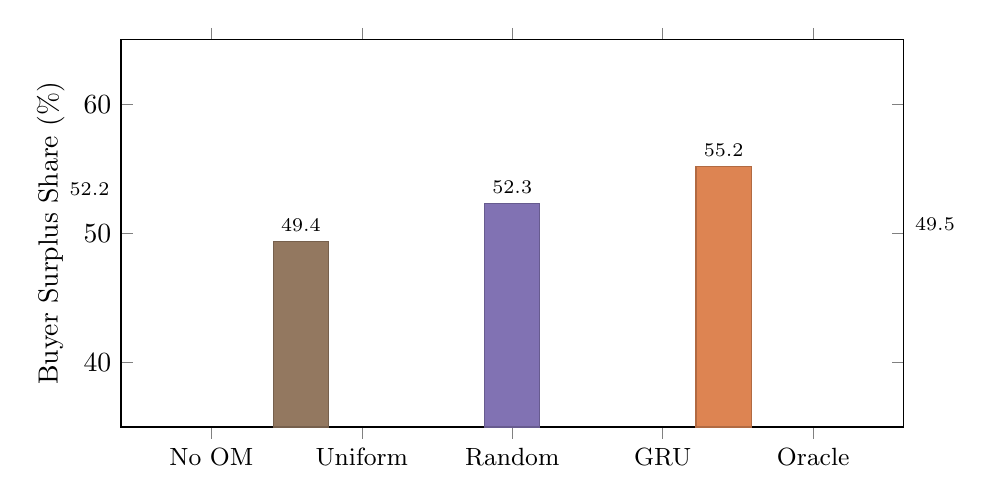
\begin{tikzpicture}
\begin{axis}[
    ybar,
    bar width=20pt,
    width=0.95\textwidth,
    height=6.5cm,
    ylabel={Buyer Surplus Share (\%)},
    symbolic x coords={No OM, Uniform, Random, GRU, Oracle},
    xtick={No OM, Uniform, Random, GRU, Oracle},
    ymin=35, ymax=65,
    nodes near coords,
    every node near coord/.append style={font=\scriptsize, /pgf/number format/fixed, /pgf/number format/precision=1},
    enlarge x limits=0.15,
    xticklabel style={font=\small},
]
\addplot[ybar, fill=condA, draw=condA!80!black] coordinates {(No OM,52.2)};
\addplot[ybar, fill=ablUniform, draw=ablUniform!80!black] coordinates {(Uniform,49.4)};
\addplot[ybar, fill=ablRandom, draw=ablRandom!80!black] coordinates {(Random,52.3)};
\addplot[ybar, fill=condB, draw=condB!80!black] coordinates {(GRU,55.2)};
\addplot[ybar, fill=ablOracle, draw=ablOracle!80!black] coordinates {(Oracle,49.5)};
\end{axis}
\end{tikzpicture}
\caption{Buyer surplus share by opponent-weight source ($N = 200$ each, randomized opener). The non-monotonic pattern reveals the Oracle Paradox: perfect information yields less buyer share than noisy predictions.}
\label{fig:ablation_bars}
\end{figure}

\begin{figure}[t]
\centering
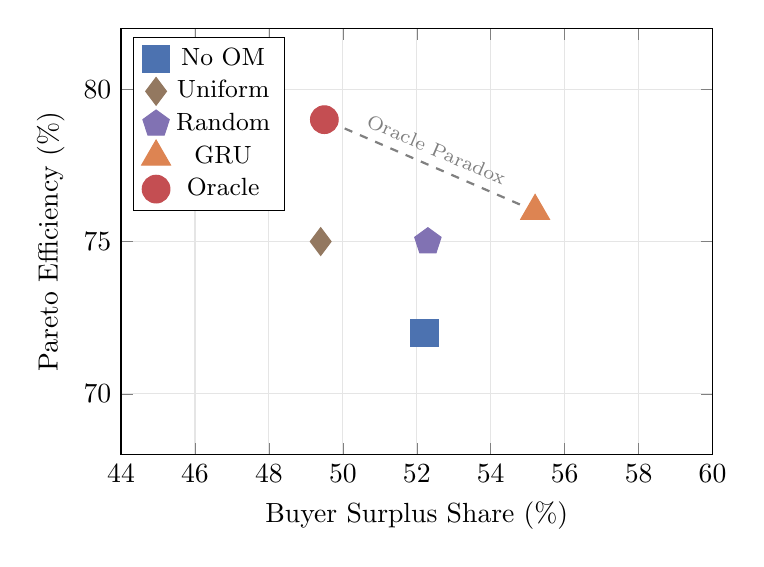
\begin{tikzpicture}
\begin{axis}[
    width=0.75\textwidth,
    height=7cm,
    xlabel={Buyer Surplus Share (\%)},
    ylabel={Pareto Efficiency (\%)},
    xmin=44, xmax=60,
    ymin=68, ymax=82,
    grid=both,
    grid style={gray!20},
    legend style={at={(0.02,0.98)}, anchor=north west, font=\small},
]
\addplot[only marks, mark=square*, mark size=5pt, condA] coordinates {(52.2, 72)};
\addplot[only marks, mark=diamond*, mark size=5pt, ablUniform] coordinates {(49.4, 75)};
\addplot[only marks, mark=pentagon*, mark size=5pt, ablRandom] coordinates {(52.3, 75)};
\addplot[only marks, mark=triangle*, mark size=6pt, condB] coordinates {(55.2, 76)};
\addplot[only marks, mark=*, mark size=5pt, ablOracle] coordinates {(49.5, 79)};
% Arrow showing the paradox
\draw[->, thick, dashed, gray] (axis cs:55.2,76) -- (axis cs:49.5,79) node[midway, above, font=\scriptsize, sloped] {Oracle Paradox};
\legend{No OM, Uniform, Random, GRU, Oracle}
\end{axis}
\end{tikzpicture}
\caption{Efficiency--distribution tradeoff ($N = 200$, randomized opener). Increasing opponent-model accuracy (GRU$\to$Oracle) improves Pareto efficiency but reduces buyer share. The arrow traces the Oracle Paradox: perfect information creates value but cannot claim it.}
\label{fig:tradeoff}
\end{figure}

\begin{figure}[t]
\centering
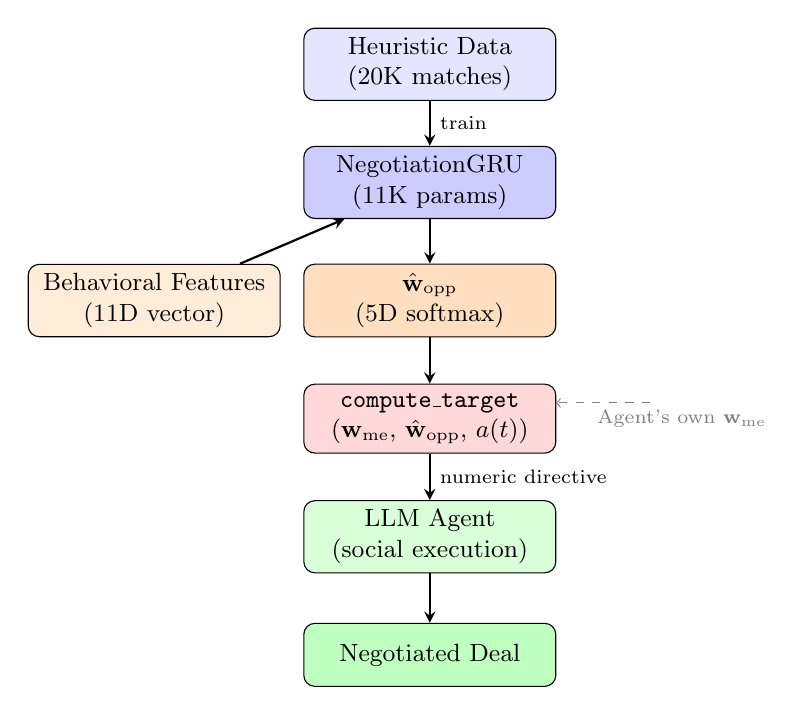
\begin{tikzpicture}[
    box/.style={draw, rounded corners, minimum width=3.2cm, minimum height=0.8cm, align=center, font=\small},
    arrow/.style={->, thick, >=stealth},
]
    \node[box, fill=blue!10] (data) at (0,4) {Heuristic Data\\(20K matches)};
    \node[box, fill=blue!20] (gru) at (0,2.5) {NegotiationGRU\\(11K params)};
    \node[box, fill=orange!15] (features) at (-3.5,1) {Behavioral Features\\(11D vector)};
    \node[box, fill=orange!25] (weights) at (0,1) {$\hat{\mathbf{w}}_\text{opp}$\\(5D softmax)};
    \node[box, fill=red!15] (target) at (0,-0.5) {\texttt{compute\_target}\\($\mathbf{w}_\text{me}$, $\hat{\mathbf{w}}_\text{opp}$, $a(t)$)};
    \node[box, fill=green!15] (llm) at (0,-2) {LLM Agent\\(social execution)};
    \node[box, fill=green!25] (deal) at (0,-3.5) {Negotiated Deal};

    \draw[arrow] (data) -- (gru) node[midway, right, font=\scriptsize] {train};
    \draw[arrow] (features) -- (gru);
    \draw[arrow] (gru) -- (weights);
    \draw[arrow] (weights) -- (target);
    \draw[arrow] (target) -- (llm) node[midway, right, font=\scriptsize] {numeric directive};
    \draw[arrow] (llm) -- (deal);

    % Self-knowledge arrow
    \node[font=\scriptsize, text=gray] at (3.2, -0.5) {Agent's own $\mathbf{w}_\text{me}$};
    \draw[->, gray, dashed] (2.8, -0.3) -- (1.6, -0.3);
\end{tikzpicture}
\caption{Computed-Target Architecture. Behavioral features extracted from the opponent's proposal trajectory are encoded by the NegotiationGRU into a 5-dimensional opponent-weight prediction $\hat{\mathbf{w}}_\text{opp}$. The \texttt{compute\_target} module blends $\hat{\mathbf{w}}_\text{opp}$ with the agent's own known weights $\mathbf{w}_\text{me}$ under an aggression schedule $a(t)$ to produce a numeric directive that the LLM executes in natural language. See \Cref{sec:opener} for the randomized-opener decomposition.}
\label{fig:architecture}
\end{figure}

% ── 7  Conclusion ─────────────────────────────────────────────────────
\section{Conclusion}
\label{sec:conclusion}

We have shown that aligned LLMs exhibit a cooperation prior that text-based strategic advice does not bypass: providing opponent-preference information as natural language consistently \emph{reduces} negotiation surplus, an effect consistent with alignment-induced cooperation bias though we do not establish this causally (see \Cref{sec:limitations}). Computed numeric targets bypass this prior by operating outside the language modality, functioning as exogenous commitment devices~\citep{schelling1960strategy} that selectively override the cooperative heuristic.

Scaled experiments ($N = 200$) and replication across eight models from five labs yield six principal findings:

\begin{enumerate}
\item \textbf{Anchoring defense ($+7.1$pp, opener-dependent).} Under seller-first opening, the computed target neutralizes first-mover anchoring. This is the largest single effect but contributes nothing when the opener is randomized.
\item \textbf{Residual GRU-conditioned share edge ($+3.0$pp, opener-independent).} At $N = 200$ under randomized opener, GRU-equipped agents outperform unassisted ones. Full ablations confirm the gradient: GRU ($55.2\%$) $>$ random ($52.3\%$) $>$ uniform ($49.4\%$) $\approx$ oracle ($49.5\%$). Combined with \Cref{sec:bias_scalar}, this is best read as a bias-conditioned target effect rather than accurate Theory-of-Mind inference. The Oracle Paradox---a mechanical consequence of the cooperative blending formula converging to Nash bargaining under perfect information---holds with $9.9\times$ variance collapse.
\item \textbf{Variance collapse ($1.1$--$2.8\times$ across the eight-model panel; $2.3$--$9.9\times$ on the Haiku $N\!=\!200$ ablation gradient, opener-independent, format-driven).} The most practically significant finding. All computed-target conditions collapse outcome standard deviation from $\pm 8.9$--$18.3\%$ to $\pm 0.9$--$4.7\%$. This enables a \emph{within-model} inference-compute arbitrage on the consistency dimension: a \$0.25/M-token model with the directive matches the outcome-stability band of frontier models. Cross-model, against frontier sellers, the cheap-with-OM stack still loses on share---so the arbitrage is consistency-bounded, not surplus-bounded.
\item \textbf{Offline channel removal closes the replayed cross-model gap and breaks the Pareto ceiling.} Replacing the LLM-to-LLM language channel with a structured middleman protocol captures $91$--$96\%$ of joint surplus (vs.\ the Oracle's $79\%$ language-channel ceiling) and reduces the $7.3$pp cross-model buyer-share spread to $\le 0.001$pp in matched-weight replay (\Cref{sec:middleman}). The cooperative-blend protocol's $50/50$ outcome is a structural property of additive opposite-direction utility and is robust to LLMIO translation noise; Nash bargaining attains the highest Pareto efficiency but is fragile to translation error. We read this as evidence consistent with a channel-mediated account of the cross-model asymmetry, while leaving live cross-model LLMIO as future work.
\item \textbf{Appendix~A reports a preliminary neural distillation result.} A 6.5K-parameter MLP trained on 660 live LLM games achieves 100\% deal rate with zero catastrophic failures and preserves the variance-collapse property without access to the hand-coded formula.
\item \textbf{At $\tau=0.2$ (single setting, not a swept result), reward-weighted regression reaches the lowest-variance policy observed.} The heuristic ($\pm 3.2\%$) and the RWR policy ($\pm 2.6\%$) are complementary operating modes: max-yield and max-safety. \emph{Critical caveat: this finding rests on one temperature value and lacks the GRU-mask control (see \Cref{sec:limitations}, items 8 and 10); we present the broader ``offline RL in stochastic multi-agent environments favors variance minimization'' claim as a hypothesis to test rather than a result established here.}
\end{enumerate}

Multi-model replication suggests a \textbf{three-tier taxonomy}: (i)~scaffold-responsive models (Grok~3, Haiku, Grok~3 Mini) gain $+3$--$7$pp buyer share with $2.0$--$2.8\times$ collapse; (ii)~collapse-only models (GPT-5, Gemini Flash, DeepSeek~R1) show $1.4$--$1.6\times$ variance reduction without surplus shift; (iii)~no detectable effect at $N\!=\!50$ for Opus~4.6 and Gemini Pro, whose baseline variance is already low (with the observed $\sigma$ values, $N\!=\!50$ resolves only effects larger than ${\sim}\pm 5$pp). Reasoning models (DeepSeek~R1) resist directives because their endogenous chain-of-thought competes with the exogenous numeric anchor.

The broader design principle: \textbf{decouple strategic computation from social execution, and remove the language channel where it is overhead}. The LLM excels as an I/O interface; the small model provides mathematically grounded guardrails; and where the conversation itself does not create value, a structured middleman protocol replaces the dialogue entirely. The two architectures span a single design axis---how much of the language channel to retain---and the choice between them is a deployment question, not a categorical one. This separation may generalize beyond negotiation to any setting where aligned LLMs must act competitively---trading agents, procurement bots, adversarial business interactions---wherever the cooperation prior or capability-driven channel exploitation conflicts with the principal's strategic objectives.

% ── Ethics statement ─────────────────────────────────────────────────
\section*{Ethics Statement}

This paper studies architectural interventions that improve the bargaining outcomes of one LLM-mediated party at the expense of another. We acknowledge the dual-use character of the work and address three specific concerns.

\paragraph{Asymmetric deployment risk.} The Computed-Target Architecture is most effective in same-population deployments where one side has the scaffold and the other does not (\Cref{tab:ablation_opener}: $+5.8$pp share gain over uniform self-knowledge at $N\!=\!200$). In a market where well-resourced parties deploy this architecture against unequipped counterparties, surplus extraction would be unilateral. We argue (\Cref{sec:middleman}) that the appropriate remedy is structural---a fair middleman protocol---rather than restricting access to the technique itself, because asymmetric defensive use (Condition C, \Cref{tab:results}) restores competitive equilibrium ($46.0\%$ buyer share, indistinguishable from $50/50$) while preserving the joint-surplus and variance benefits.

\paragraph{Consumer protection in agent-to-agent commerce.} \emph{Project Deal}~\citep{anthropic2026projectdeal} reports that users represented by weaker models received objectively worse outcomes than users represented by stronger models, while reporting indistinguishable fairness ratings ($4.05$ vs.\ $4.06$). Our Middleman Protocol results (\Cref{sec:middleman}) are consistent with the interpretation that much of this asymmetry is expressed through the language channel rather than through an immutable capability gap: replacing the channel with a structured numeric protocol collapses the replayed cross-model surplus spread to $\le 0.001$pp. We frame this as a design opportunity for marketplace operators, clearinghouses, and regulators: the entity running the equivalent of a fair-protocol layer is making a substantive distributional choice. This framing is descriptive; we do not advocate for any specific regulatory regime.

\paragraph{No human subjects, no PII.} All experiments involved only LLM agents in a synthetic 5-variable B2B SaaS contract environment with Dirichlet-sampled utility weights. No real user data, no real commercial transactions, and no identifiable preferences appear in the bundled data packet.

% ── Acknowledgments ──────────────────────────────────────────────────
\section*{Acknowledgments}

The author received no external funding for this work and reports no competing interests. All inference was paid out of pocket via OpenRouter API credit. Thanks to the maintainers of the open-source Python scientific stack (PyTorch, NumPy, SciPy, scikit-learn) and to OpenRouter for providing a unified interface to the eight LLMs under test, which materially reduced the engineering surface of multi-model replication. Any errors of analysis or interpretation are the author's alone.

% ── References ────────────────────────────────────────────────────────
\section*{References}
\begingroup
\renewcommand{\section}[2]{}
\begin{thebibliography}{99}

\bibitem[Abdelnabi et~al.(2024)]{abdelnabi2024cooperation}
S.~Abdelnabi, A.~Gomaa, S.~Sivaprasad, M.~Sch{\"o}nherr, and M.~Fritz.
\newblock Cooperation, competition, and maliciousness: {LLM}-stakeholders interactive negotiation.
\newblock \emph{arXiv preprint arXiv:2309.17234}, 2024.

\bibitem[Anthropic(2026)]{anthropic2026projectdeal}
Anthropic.
\newblock Project {D}eal: An experimental agent-to-agent marketplace.
\newblock \url{https://www.anthropic.com/features/project-deal}, 2026.
\newblock Accessed 2026-04-26.

\bibitem[Baarslag et~al.(2013)]{baarslag2013acceptance}
T.~Baarslag, K.~Hindriks, and C.~Jonker.
\newblock Acceptance conditions in automated negotiation.
\newblock In \emph{Complex Automated Negotiations}, pages 95--111. Springer, 2013.

\bibitem[Baarslag et~al.(2015)]{baarslag2015anac}
T.~Baarslag, M.~Hendrikx, K.~Hindriks, and C.~Jonker.
\newblock Learning about the opponent in automated bilateral negotiation: A comprehensive survey of opponent modeling techniques.
\newblock \emph{Autonomous Agents and Multi-Agent Systems}, 30(5):849--898, 2015.

\bibitem[Bakhtin et~al.(2022)]{bakhtin2022human}
A.~Bakhtin, N.~Brown, E.~Dinan, G.~Farina, C.~Flaherty, D.~Fried, A.~Goff, J.~Gray, H.~Hu, et~al.
\newblock Human-level play in the game of {D}iplomacy by combining language models with strategic reasoning.
\newblock \emph{Science}, 378(6624):1067--1074, 2022.

\bibitem[Bianchi et~al.(2024)]{bianchi2024llm}
F.~Bianchi, P.~Chia, M.~Yuksekgonul, J.~Tagliabue, D.~Jurafsky, and J.~Zou.
\newblock How well can {LLM}s negotiate? {NegotiationArena} platform and analysis.
\newblock \emph{arXiv preprint arXiv:2402.05863}, 2024.

\bibitem[Davidson et~al.(2024)]{davidson2024evaluating}
T.~R. Davidson, V.~Veselovsky, M.~Kosinski, and R.~West.
\newblock Evaluating language model agency through negotiations.
\newblock In \emph{International Conference on Learning Representations (ICLR)}, 2024.

\bibitem[Fu et~al.(2023)]{fu2023improving}
Y.~Fu, H.~Peng, L.~Ou, A.~Sabharwal, and T.~Khot.
\newblock Improving language model negotiation with self-play and in-context learning from {AI} feedback.
\newblock \emph{arXiv preprint arXiv:2305.10142}, 2023.

\bibitem[Gandhi et~al.(2023)]{gandhi2023strategic}
K.~Gandhi, D.~Sadigh, and N.~D.~Goodman.
\newblock Strategic reasoning with language models.
\newblock \emph{arXiv preprint arXiv:2305.19165}, 2023.

\bibitem[Garc{\'e}z and Lamb(2023)]{garcez2023neurosymbolic}
A.~d'Avila~Garc{\'e}z and L.~C.~Lamb.
\newblock Neurosymbolic {AI}: The 3rd wave.
\newblock \emph{Artificial Intelligence Review}, 56:12387--12406, 2023.

\bibitem[He et~al.(2018)]{he2018decoupling}
H.~He, D.~Chen, A.~Balakrishnan, and P.~Liang.
\newblock Decoupling strategy and generation in negotiation dialogues.
\newblock In \emph{Empirical Methods in Natural Language Processing (EMNLP)}, 2018.

\bibitem[Kasparov(2017)]{kasparov2017deep}
G.~Kasparov.
\newblock \emph{Deep Thinking: Where Machine Intelligence Ends and Human Creativity Begins}.
\newblock PublicAffairs, 2017.

\bibitem[Lax and Sebenius(1986)]{lax1986manager}
D.~A. Lax and J.~K. Sebenius.
\newblock \emph{The Manager as Negotiator}.
\newblock Free Press, 1986.

\bibitem[Lewis et~al.(2017)]{lewis2017deal}
M.~Lewis, D.~Yarats, Y.~Dauphin, D.~Parikh, and D.~Batra.
\newblock Deal or no deal? End-to-end learning for negotiation dialogues.
\newblock In \emph{Empirical Methods in Natural Language Processing (EMNLP)}, 2017.

\bibitem[Nash(1950)]{nash1950bargaining}
J.~Nash.
\newblock The bargaining problem.
\newblock \emph{Econometrica}, 18(2):155--162, 1950.

\bibitem[Park et~al.(2024)]{park2024ai}
P.~S. Park, S.~Goldstein, A.~O'Gara, M.~Chen, and D.~Hendrycks.
\newblock {AI} deception: A survey of examples, risks, and potential solutions.
\newblock \emph{Patterns}, 5(5):100988, 2024.

\bibitem[Perez et~al.(2022)]{perez2022discovering}
E.~Perez, S.~Ringer, K.~Luko\v{s}i\={u}t\.{e}, K.~Nguyen, et~al.
\newblock Discovering language model behaviors with model-written evaluations.
\newblock \emph{arXiv preprint arXiv:2212.09251}, 2022.

\bibitem[Peters and Schaal(2007)]{peters2007reinforcement}
J.~Peters and S.~Schaal.
\newblock Reinforcement learning by reward-weighted regression for operational space control.
\newblock In \emph{International Conference on Machine Learning (ICML)}, 2007.

\bibitem[Rabinowitz et~al.(2018)]{rabinowitz2018machine}
N.~Rabinowitz, F.~Perbet, H.~F.~Song, C.~Zhang, S.~M.~A.~Eslami, and M.~Botvinick.
\newblock Machine theory of mind.
\newblock In \emph{ICML}, 2018.

\bibitem[Raiffa(1982)]{raiffa1982art}
H.~Raiffa.
\newblock \emph{The Art and Science of Negotiation}.
\newblock Harvard University Press, 1982.

\bibitem[Schelling(1960)]{schelling1960strategy}
T.~C. Schelling.
\newblock \emph{The Strategy of Conflict}.
\newblock Harvard University Press, 1960.

\bibitem[Schick et~al.(2023)]{schick2023toolformer}
T.~Schick, J.~Dwivedi-Yu, R.~Dess{\`i}, et~al.
\newblock Toolformer: Language models can teach themselves to use tools.
\newblock In \emph{NeurIPS}, 2023.

\bibitem[Sharma et~al.(2023)]{sharma2023sycophancy}
M.~Sharma, M.~Tong, T.~Korbak, D.~Duvenaud, A.~Askell, et~al.
\newblock Towards understanding sycophancy in language models.
\newblock \emph{arXiv preprint arXiv:2310.13548}, 2023.

\bibitem[Wang et~al.(2022)]{wang2022tom2c}
Y.~Wang, F.~Zhou, B.~Liu, P.~Li, X.~Ma, Y.~Wang, H.~Dong, S.-C. Zhu, and Y.~Zhu.
\newblock {ToM2C}: Target-oriented multi-agent communication and cooperation with theory of mind.
\newblock In \emph{International Conference on Learning Representations (ICLR)}, 2022.

\end{thebibliography}
\endgroup

% ── Appendix A: Neural Policy Learning ───────────────────────────────
\appendix

\section{Distilling the Guardrail Architecture}
\label{sec:policy}

This appendix describes a follow-on study, conducted after the headline experiments, that asks whether the low-variance behavior of the computed-target architecture can be amortized into a small neural policy trained on LLM telemetry rather than expressed by a hand-coded formula. The result is a hypothesis, not a load-bearing claim of the main paper: a 6.5K-parameter MLP trained via reward-weighted regression at $\tau\!=\!0.2$ converged to the lowest-variance policy we observed, but the convergence claim rests on a single temperature setting and one of its key controls (a GRU-feature mask) was not run. We include it here for completeness and because the variance-vs-yield tradeoff it surfaces is itself useful for downstream readers.

The computed-target formula (\Cref{eq:target,eq:blend}) is hand-coded for a 5-variable game. Real-world multi-issue contracts involve dozens of interrelated terms where closed-form solutions are infeasible. We ask: can a neural network \emph{distill} this architecture's behavior from LLM game telemetry, bypassing the hand-coded math at deployment time?

\subsection{Architecture and State Representation}

We train a \textbf{NegotiationPolicyNet} ($6{,}533$ parameters): a 3-layer MLP mapping a 27-dimensional state vector to a 5D proposal, clamped to $[0.05, 0.95]$. The architecture is Linear($27\!\to\!64$)$\to$LayerNorm$\to$GELU$\to$Linear($64\!\to\!64$)$\to$LayerNorm$\to$GELU$\to$Linear($64\!\to\!5$):

\begin{equation}
\pi_\theta: \mathbb{R}^{27} \to [0.05, 0.95]^5
\label{eq:policy}
\end{equation}

The 27D state comprises the agent's own weights (5D), round fraction (1D), opponent's latest proposal (5D), utilities at current offers (2D), agent's latest proposal (5D), opponent proposal count (1D), role indicator (1D), briefing indicator (1D), opponent concession rate (1D), and the GRU-predicted opponent weights (5D). Because the training data is generated by the GRU-mediated architecture later reframed in \Cref{sec:bias_scalar} as a bias-equipped numeric sub-agent, this appendix should be read as a distillation study rather than as evidence that the network discovered negotiation strategy from scratch. Whether the policy actually relies on the GRU's 5 dimensions rather than the 22 base features is a question we did not run as a controlled ablation (see Limitation 10 in \Cref{sec:limitations}); claims in this appendix should be read with that caveat in mind.

\subsection{Training Methods}

We extract $4{,}341$ state-action-reward tuples from 660 live Haiku-vs-Haiku negotiation games drawn from the seller-first Condition~B run (\Cref{tab:results}) and from $N\!=\!50$ randomized-opener ablation conditions (B+GRU, B+Uniform, B+Random, B+Oracle). Games are split at the \emph{game} level (not the tuple level) into train/validation to prevent within-game leakage. The exact game $\to$ split assignment is reproducible from \texttt{seeds.json} in the data packet.

\paragraph{Behavioral Cloning (BC).} Filter for top-quartile games by agent utility ($\geq 0.653$, yielding 914 samples). Minimize weighted MSE: $\mathcal{L}_\text{BC} = \sum_i w_i \|\pi_\theta(s_i) - a_i\|^2$, where $w_i$ is the normalized utility. Adam optimizer, lr $= 3 \times 10^{-4}$, cosine annealing, early stopping (patience 10).

\paragraph{Reward-Weighted Regression (RWR)~\citep{peters2007reinforcement}.} Use all data. Weight each sample by $\exp(\text{advantage}_i / \tau)$ where $\text{advantage}_i = r_i - \bar{r}$, $\bar{r}$ is the global mean buyer utility over all 4{,}341 training tuples, and temperature $\tau = 0.2$. This upweights the highest-reward trajectories (max weight $5.4\times$), biasing the policy toward the most successful negotiations in the dataset.

\subsection{Live A/B Test Results}

Both models are evaluated via live A/B test: 50 games per condition, randomized opener, Claude 3.5 Haiku, against the heuristic baseline from \Cref{sec:computed}.

\begin{table}[t]
\centering
\caption{Live A/B test results ($N = 50$ per condition, randomized opener, Claude 3.5 Haiku). Condition~A baseline ($N = 200$) shown for reference. The heuristic maximizes yield ($56.2\%$); the RWR neural policy minimizes variance ($\pm 2.6\%$). Both beat the unassisted baseline with 100\% deal rate.}
\label{tab:policy_ab}
\begin{tabular}{lcccc}
\toprule
Metric & A (No OM) & B-heuristic & B-policy (BC) & B-policy (RWR) \\
\midrule
Deal rate & 100\% & 100\% & 100\% & 100\% \\
Buyer share (mean) & 52.2\% & \textbf{56.2\%} & 53.3\% & 53.9\% \\
Buyer share ($\sigma$) & $\pm$ 8.9\% & $\pm$ 3.2\% & $\pm$ 4.5\% & $\pm$ \textbf{2.6\%} \\
95\% CI & --- & [55.3, 57.1] & [52.0, 54.6] & [53.2, 54.7] \\
Pareto efficiency & 72\% & 76\% & 75\% & 76\% \\
$\Delta$ vs baseline & --- & $+4.0$pp & $+1.1$pp & $+1.7$pp \\
\bottomrule
\end{tabular}
\end{table}

\subsection{The Imitation Ceiling}

Neither model surpasses the heuristic in mean buyer share. This is expected: behavioral cloning is mathematically bounded by the expert it imitates. The dataset was largely generated by the heuristic, so the BC model can at best replicate it. Getting within 2.9pp of a hand-crafted formula purely by observing text transcripts---without access to the formula itself---validates the neural architecture as a distillation target. The key insight, however, is that the RWR policy \emph{does} surpass the heuristic on variance ($\pm 2.6\%$ vs $\pm 3.2\%$), offering a distinct operating mode for risk-sensitive deployments.

\subsection{The Variance--Reward Tradeoff}
\label{sec:vault}

The RWR result is the experiment's most notable finding. We set $\tau = 0.2$, upweighting top performers by up to $5.4\times$, explicitly biasing the policy toward high-reward trajectories. Rather than producing a more aggressive policy, the network converged to the lowest-variance model tested in this research:

\begin{table}[h]
\centering
\caption{Variance-reward tradeoff across all architectures. The heuristic maximizes yield ($56.2\%$); the RWR neural policy minimizes variance ($\pm 2.6\%$), below the heuristic ($\pm 3.2\%$), at a cost of $-2.3$pp in mean buyer share.}
\label{tab:vault}
\begin{tabular}{lcc}
\toprule
Model & Buyer share (mean) & Buyer share ($\sigma$) \\
\midrule
No OM (baseline) & 52.7\% & $\pm$ 8.1\% \\
Heuristic (max yield) & 56.2\% & $\pm$ 3.2\% \\
BC neural policy & 53.3\% & $\pm$ 4.5\% \\
\textbf{RWR neural policy (max safety)} & \textbf{53.9\%} & $\pm$ \textbf{2.6\%} \\
\bottomrule
\end{tabular}
\end{table}

The mechanism is instructive. In a deterministic game (e.g., chess), upweighting the highest rewards makes an agent more aggressive. But in a stochastic environment---where the opponent is a live LLM with variable RLHF-induced cooperation levels---the rare high-surplus games in the training data are not attributable to a repeatable strategy. They occurred because the opposing LLM happened to be unusually pliable. Attempting to replicate those ``Shark'' moves against every opponent risks triggering the walk-away threshold and collapsing the deal.

The RWR network's effective optimum is therefore conservative: maximize expected value across all stochastic opponents by avoiding tail risks. The policy converges to a $53.9\%$ mean with $\pm 2.6\%$ variance rather than attempting to reach the heuristic's $56.2\%$ mean with $\pm 3.2\%$ variance. These are not a ``winner'' and a ``loser''---they are two distinct operating modes: the heuristic is a max-yield engine; the RWR policy is a max-safety engine.

\paragraph{Implication (with caveat).} In standard RL, low-temperature RWR is known to cause \emph{mode collapse}---the policy drops entropy and collapses to the mean of a few high-reward trajectories, which is typically undesirable. In the context of enterprise LLM negotiation, mode collapse may instead be desirable: it would act as an algorithmic safety mechanism that crushes outcome variance and produces a hyper-conservative, deployable policy. This is suggestive of a broader claim---that offline RL in stochastic multi-agent environments may favor variance minimization over reward maximization---but our evidence is one $\tau$ ($0.2$) on one task. We have not swept temperature, varied dataset composition, or replicated on another domain. Read the result as a hypothesis to test, not a property established here. If the mechanism is real, the explanation is intuitive: when high-reward outcomes in the training data are attributable to opponent stochasticity rather than repeatable strategy, reward-weighted optimization learns to avoid the high-variance actions that produced those outcomes, because the associated risks (deal collapse, reward $= 0$) dominate in expectation.

\subsection{What This Appendix Does and Does Not Show}

The neural policy's significance is not that it beats the heuristic---it does not. Three narrower observations stand without the temperature sweep or the GRU-mask control:

\begin{enumerate}
\item \textbf{Sim-to-real crossing.} A neural network trained on offline telemetry successfully negotiates against live LLMs at $100\%$ deal rate without catastrophic out-of-distribution failures.
\item \textbf{Variance preservation.} The learned model preserves the variance-collapse property of the computed-target architecture without access to the hand-coded formula.
\item \textbf{Scalability path.} One can write a closed-form heuristic for 5 variables. One cannot for a 50-variable multi-issue contract. The fact that an MLP can distill the architecture's behavior from behavioral telemetry alone is suggestive evidence that the approach extends beyond hand-coded formulas, though the strength of that evidence is bounded by the controls we did not run.
\end{enumerate}

\end{document}
